\documentclass{article}

\usepackage{amsmath}
\usepackage{amsthm}
\usepackage{amssymb}
\usepackage{graphicx}
\usepackage{diagbox}

\graphicspath{{pics/}}

%CURLIES  :)       $\{$ $\}$

\newcommand{\ti}[1]{\textit{#1}}
\newcommand{\tb}[1]{\textbf{#1}}
\newcommand{\N}{\mathbb{N}}
\newcommand{\Z}{\mathbb{Z}}
\newcommand{\Q}{\mathbb{Q}}
\newcommand{\R}{\mathbb{R}}
\newcommand{\C}{\mathbb{C}}
\newcommand{\bbP}{\mathbb{P}}
\newcommand{\bbE}{\mathbb{E}}
\newcommand{\Om}{\Omega}
\newcommand{\om}{\omega}
\newcommand{\la}{\lambda}
\newcommand{\ep}{\varepsilon}
\newcommand{\emp}{\emptyset}
\newcommand{\lt}{\textless}
\newcommand{\gt}{\textgreater}
\newcommand{\imply}{\Rightarrow}
\newcommand{\x}{\cdot}
\newcommand{\Ga}{\Gamma}
\newcommand{\al}{\alpha}
\newcommand{\sg}{\sigma}
\newcommand{\be}{\beta}
\newcommand{\prop}{\textbf{Proposition: }}
\newcommand{\thm}{\textbf{Theorem: }}
\newcommand{\lem}{\textbf{Lemma: }}
\newcommand{\cor}{\textbf{Corollary: }}
\newcommand{\proo}{\textbf{Proof: }}
\newcommand{\exx}{\textbf{Ex: }}
\newcommand{\exxi}{\textbf{Ex 1: }}
\newcommand{\exxii}{\textbf{Ex 2:  }}
\newcommand{\exxiii}{\textbf{Ex 3:  }}
\newcommand{\soln}{\textbf{Solution: }}

\title{MATH 323 Class Notes}
\author{Owen Lewis}
\date{Summer 2018}

\begin{document}
\begin{titlepage}
\maketitle
\end{titlepage}

\tableofcontents
\newpage

%%%%%%%%%%%%%%%%%%%%%%%%%%%%%%%%%%%%%%%%%%%%%%%%%%%%%%%%%%%%%%%%%%%%%%

\section{May 1, 2018}
\subsection{Definitions}
Let $\Omega$ be the set of all possible outcomes. We call $\Omega$ the $\ti{Sample Space}$.\\\\
\textbf{Ex 1:} Flipping a coin. The possible outcomes are $H$ and $T$\\
$\imply$ $\Omega$ = $\{$$H$, $T$$\}$.\\
\textbf{Ex 2:} Tossing a die. We list all the outcomes as $\omega_{i}$ where $i$ is the face of the die that we land on. We'll assume a normal 6-sided die\\ 
$\imply$ $\Omega$ = $\{$$\omega_{1}$, $\omega_{2}$,\dots, $\omega_{6}$$\}$.\\
\textbf{Ex 3:} Flipping a coin until an $H$ appears. The possible outcomes are $H$, $TH$, $TTH$,\dots, $TT$$\dots$$TH$ (with $n-1$ $T$s), $\dots$ ad infinitum.\\\\
$\imply$ $\Omega$ = $\{$$H, TH, TTH, TTTH, TTTTH,\dots$$\}$.\\
Note that in this case, $\Omega$ is a (countably) infinite set!\\\\
Let $\Omega$ be a sample space. Any subset $A$ of $\Omega$ is called an $\it{Event}$.
\begin{itemize}
	\item If $A$ = $\emptyset$, then we call $A$ the $\ti{Null Event}$
	\item If $A$ = $\Omega$, then we call $A$ the $\ti{Certain Event}$
	\item If $|$$A$$|$ = 1, then we call $A$ an $\ti{Elementary Event}$
\end{itemize}
\textbf{Ex:} Tossing a die. Let $\Omega$ := $\{$$\omega_{1}$, $\omega_{2}$,\dots, $\omega_{6}$$\}$, $A$ := $\{$$\omega_{1}$, $\omega_{2}$$\}$. Then $A$ is an event but is not an elementary event.\\\\
If $A$ is an event, then $A^{c}$ is also an event called the $\ti{complement event}$ of $A$.\\
If $A, B$ are two disjoint events then we call $A$, and $B$ $\ti{mutually exclusive}$, or $\ti{disjoint}$.\\\\
Let $\Omega$ be a sample space, $\mathcal{P}$ be the power set of $\Om$. A $\ti{Probability}$ $\bbP$ on $\Om$ is a function $\bbP$ : $\mathcal{P}$($\Om$) $\rightarrow$ [0, 1], such that:
\begin{enumerate}
	\item $\forall$ $A$ $\subseteq$ $\Om$, 0 $\leq$ $\bbP$($A$) $\leq$ 1
	\item $\bbP$($\Om$) = 1
	\item If $A_{1}$, $A_{2}$,\dots, $A_{n}$,\dots\ is a sequence of pairwise disjoint events then
\[ \bbP(\bigcup_{i=1}^{\infty} p_{i}) = \sum_{i=0}^{\infty} \bbP(A_{i}) \]
\end{enumerate}
\newpage
\subsection{How do we Apply this?}
Let $\Om$ be a discrete set, $E_{i}$ = $\{$$\omega_{i}$$\}$ be an elemental event, with $E_{i}$ $\subseteq$ $\Om$. A probability on $\Om$ is given by a sequence $\bbP_{1}$, $\bbP_{2}$,\dots, $\bbP_{n}$,\dots of positive numbers such that
\[ \bbP(E_{i}) = p_{i},\ and\ \sum_{i} \bbP(p_{i}) = 1\]\\
If $A$ $\subseteq$ $\Om$, then
\[ \bbP(A) = \sum_{\omega_{i} \in A} \bbP(p_{i})\]\\
\textbf{Ex 1:} Toss a die.\\
a) Given that $\bbP$($\omega_{2}$) = $\bbP$($\omega_{4}$) = $\bbP$($\omega_{5}$) = $\bbP$($\omega_{6}$) = $\frac{1}{6}$, $\bbP$($\omega_{1}$) = $\frac{1}{4}$, find $\bbP$($\omega_{3}$).\\
b) Find the probability that the die will land on an odd face.\\
\textbf{Solution:}\\
a) $\Omega$ = $\{$$\omega_{1}$, $\omega_{2}$,\dots, $\omega_{6}$$\}$. $\bbP$($\omega_{3}$) is a singleton, and as we know $\sum_{i} \bbP(p_{i})$ = 1 then  $\sum_{i=1}^{6}\bbP(\omega_{i})$ = 1 $\implies$ $\bbP$($\omega_{2}$) + $\bbP$($\omega_{4}$) + $\bbP$($\omega_{5}$) + $\bbP$($\omega_{6}$) + $\bbP$($\omega_{1}$) + $\bbP$($\omega_{3}$) = 1 $\implies$ $\frac{4}{6}$ + $\frac{1}{4}$ + $\bbP$($\omega_{3}$) = 1 $\implies$ $\bbP$($\omega_{3}$) = 1 - $\frac{11}{12}$\\
$\implies$ $\bbP$($\omega_{3}$) = $\frac{1}{12}$.\\
b) Let $A$ $\subseteq$ $\Om$ be the subset of $\Om$ containing all the odd faces. The total probablilty of $A$ is therefore the sum of all the probabilities of the elements of $A$ $\imply$ $\bbP$($A_{i}$) = $\frac{1}{4}$ + $\frac{1}{12}$ + $\frac{1}{6}$ = $\frac{1}{2}$.\\\\
\textbf{Ex 2:} Given a countably infinite sample space, find a constant $c$ such that $\bbP$($\{$$\omega_{n}$$\}$) = $c(\frac{1}{5})^n$ for some $n$.\\
\textbf{Solution:} $\sum_{n=1}^{\infty} \bbP$($\{$$\omega_{n}$$\}$) = 1 $\imply$ $\sum_{n=1}^{\infty} c(\frac{1}{5})^n$ = 1 $\imply$ $\sum_{n=1}^{\infty} (\frac{1}{5})^n$ = $\frac{1}{c}$. Notice how $\sum_{n=1}^{\infty} (\frac{1}{5})^n$ is a geometric series that converges to $\frac{1}{4}$ $\imply$ therefore $\frac{1}{c}$ = $\frac{1}{4}$\\
$\imply$ $c$ = 4.
\newpage

%%%%%%%%%%%%%%%%%%%%%%%%%%%%%%%%%%%%%%%%%%%%%%%%%%%%%%%%%%%%%%%%%%%%%%

\section{May 2, 2018}
\subsection{Properties of $\bbP$}
Let $\Om$ be a sample space and let $\bbP$ be a probability on $\Om$. Then:
\begin{enumerate}
	\item $\bbP$($\emptyset$) = 0
	\item $\bbP$($A^{c}$) = 1 - $\bbP$($A$)
	\item $\bbP$($A \cup B$) = $\bbP(A)$ + $\bbP(B)$ - $\bbP(A \cap B)$
\end{enumerate}
Proof:
\begin{enumerate}
	\item Set $A_{1}$ = $\Om$, $A_{2}$ = $\emp$. Then $A_{1} \cup A_{2}$ = $\Om$, and $A_{1} \cap A_{2}$ = $\emp$. Therefore $\bbP(A_{1} \cup A_{2}$) = $\bbP(A_{1})$ + $\bbP(A_{2})$ $\imply$ $\bbP(\Om)$ = $\bbP(\emp)$ + $\bbP(\Om)$ $\imply$ 1 = $\bbP(\emp)$ + 1\\ $\imply$ 0 = $\bbP(\emp)$. \qed

	\item $A^{c} \cup A$ = $\Om$, and $A^{c} \cap A$ = $\emp$. Then = $\bbP(\Om)$ $\imply$ 1 = $\bbP(A^{c} \cup A)$\\ $\imply$ 1 = $\bbP(A)$ + $\bbP(A^{c})$ $\imply$ $\bbP(A^{c})$ = 1 - $\bbP(A)$. \qed

	\item It's easy to show that $A$ = $(A \setminus B) \cup (A \cap B)$, and $\emp$ = $(A \setminus B) \cap (A \cap B)$. Similarily, $\bbP(A)$ = $\bbP(A \setminus B)$ + $\bbP(A \cap B)$. From these, it follows that\\ $A \cup B$ = $A \cup (B \setminus A)$ $\imply$ $\bbP(A \cup B)$ = $\bbP(A)$ + $\bbP(B \setminus A)$\\ $\imply$ $\bbP$($A \cup B$) = $\bbP(A)$ + $\bbP(B)$ - $\bbP(A \cap B)$. \qed
\end{enumerate}

\subsection{Equiprobability}
Let $\Om$ be a finite sample space. Set $N$ := $|\Om|$. Equiprobability means that all outcomes have the same probability $\bbP$ = $\frac{1}{N}$. Let $A \subseteq \Om$ be an event. Then we have $\bbP(A)$ = $|A|$$\cdot$$\frac{1}{N}$, or 
\[\bbP(A) = \frac{|A|}{|\Om|}\]
This is great because it means that in \textbf{equiprobability} problems we just need to count the cardinality of $A$, count the cardinality of $\Om$, and divide them, and we're done. Too bad counting isn't really all that easy.

\subsection{Counting Tools}
We have here three tools to help us calculate the cardinalities of huge (finite) subsets of huge sample spaces, each with their own specific situations that require its use
\begin{enumerate}
	\item The Cartesian Product
	\item Permutations
	\item Combinations
\end{enumerate}
\subsubsection{The Cartesian Product}
\paragraph{}
We all know what the cartesian product $is$. In probability we use it in our experiment when we have more than one """input""" each with its own possible outcome, for example, we roll three dice, or flip two coins.
\paragraph{}
Let $A$, $B$, be sets such that $|A|$ = $a$, and $|B|$ = $b$. Then the cardinality of the cartesian product $|(A \times B)|$ is $|(A \times B)|$ = $a \cdot b$.\\\\
\textbf{Ex 1:} Suppose we roll a die twice. What is the cardinality of the sample space $\Om$?\\
\textbf{Solution:} If we roll a die once we have $\Om$ = $\{$$\omega_{1}$, \dots, $\omega_{6}$$\}$. Therefore, the sample space for rolling a die twice is $\Om \times \Om$. The cardinality of our sample space $\Om \times \Om$ is $|\Om \times \Om|$ = 6 $\cdot$ 6 = 36.\\\\
\textbf{Ex 2:} Suppose we roll a fair die twice. What is the probability that the outcome is even?\\
\textbf{Solution:} If the sum of the two outcomes is even then both must either be even or both must be odd. Let $A$ be the event where the sum of the rolls is even, and let $A_{1}$ be event where both individual rolls are even, $A_{2}$ be the event where both individual rolls are odd. For example,
\[A_{1} = \{(2, 2), (2, 4), (2, 6), (4, 2), (4, 4), (4, 6), (6, 2), (6, 4), (6, 6)\}\] 
Where the 1$^{st}$ element in each ordered pair is the outcome of the 1$^{st}$ roll and the 2$^{nd}$ element in each ordered pair is the outcome of the 2$^{nd}$ roll. Therefore, we have that $|A_{1}|$ = $|A_{2}|$ = 9.\\ 
Since naturally $A$ = $A_{1} \cup A_{2}$ then $\bbP(A)$ = $\bbP(A_{1})$ + $\bbP(A_{2})$. We also know that the die was fair, so we can use our equiprobability formula here.
\[ \bbP(A) = \bbP(A_{1}) + \bbP(A_{2}) = \frac{|A_{1}|}{|\Om|} + \frac{|A_{2}|}{|\Om|} = \frac{9}{36} + \frac{9}{36} = \frac {18}{36} = \frac{1}{2}.\]
\subsubsection{Permutations}
A permutation of $r$ integer elements chosen from $n$ (possible elements) is equivalent to a successive draw, without replacement, of $r$ elements from a list of $n$ elements. We denote the number of possibilities by $P_{r}^{n}$. The general formula for $P_{r}^{n}$ is
\[P_{r}^{n} = n \cdot (n-1) \cdot \dots \cdot (n-r+1) = \frac{n!}{(n-r)!}\]\\
\textbf{Ex:} \\
a) A thick black bag contains 4 balls: 1 green, 1 blue, 1 red, 1 yellow. The bag is made of lead, or something, and also light cannot exist in this bag. You couldn't see into this bag if your life depended on it. Draw successively two balls from the bag without putting them back in. What is the probability that the second ball drawn is green?\\
b) What is the probability that one of the two balls drawn will be green?\\
\textbf{Solution:}\\
a) Let $\Om$ be the set of permutations of 2 balls chosen from the bag containing 4 balls. Then, $|P^{4}_{2}|$ = $\frac{4!}{2!}$ = $\frac{24}{2}$ = 12. Then let $A$ be the event where the second ball is green. The cardinality of $A$ is 3, as if we take for granted that the second ball is green, then there are 3 other different-coloured balls in the bag to accompany it. Since the bag is so dark that it's physically impossible to see inside it, all the balls in the bag have an equal probability of being drawn. Therefore,
\[ \bbP(A) = \frac{|A|}{|\Om|} = \frac{3}{12} = \frac{1}{4}\]
b) Let $B$ be the event where one of the balls drawn is green. Suppose $B_{1}$ is the event where the first ball drawn is green, and $B_{2}$ is the event where the second ball drawn is green. In part a) we found that $|B_{2}|$ = 3, and a parallel argument shows that $|B_{2}|$ = 3 as well. Thus,
 \[ \bbP(B) = \frac{|B_{1}|}{|\Om|} + \frac{|B_{2}|}{|\Om|} = \frac{3}{12} + \frac{3}{12} = \frac{6}{12} = \frac{1}{2}\]
\subsubsection{Combinations}
Consider a set $\Om$ with $n$ elements. Let $r$ be an integer such that $0 \leq r \leq n$. A combination $C^{n}_{r}$, also denoted ${n}\choose{r}$ (pronounced $n$ choose $r$), is the number of subsets of $\Om$ containing $r$ elements. The general formula is
\[C^{n}_{r} = \frac{P_{n}^{r}}{r!} = \frac{n!}{r! \cdot (n-r)!}\]
\textbf{Ex:}\\
a) Out of a deck of 52 cards how many distinct 5-card hands are possible?\\
b) What is the probability that a given hand contains at least one ace?\\
\textbf{Solution:}\\
a) ${52}\choose{5}$ = $\frac{52!}{5! \cdot (47!)}$ = 2,598,960\\
b) In this case it is easier to calculate the probability where the hand contains no aces and then subtract that from 1 to find the probability that we have an ace. If $A$ is the event where the hand contains an ace, then $A^{c}$ is the event where a hand contains no ace. Then
\[\bbP(A^{c}) =  \frac{|A^{c}|}{|\Om|} = \frac{C^{48}_{5}}{C^{52}_{5}} = \frac{1,712,304}{2,598,960} = \frac{35,673}{54,145}\]
Then we need to subtract this from 1 and we're done
\[\bbP(A) = 1 - \frac{35,673}{54,145} \approx 0.3412\]
\subsection{Properties of Combinations}
Here are some properties of combinations
\begin{enumerate}
	\item $C^{n}_{0}$ = $C^{n}_{n}$ = 1
	\item $C^{n}_{r}$ = $C^{n}_{n-r}$ $0 \leq r \leq n$
	\item $C^{n}_{r}$ = $C^{n-1}_{r}$ + $C^{n-1}_{r-1}$ $0 \leq r \leq n$
\end{enumerate}
The proofs are really easy and I dont wan't to bother typing them out but here is the idea behind each of them:
\begin{enumerate}
	\item Trivial
	\item Induction on $n$
	\item Also induction on $n$
\end{enumerate}
\subsubsection{Pascal's Triangle}
Pascal's triangle is a table of combinations $C_{r}^{n}$. The rows of the triangle represent $n$, starting at 0 at the tip and working down, and the $r^{th}$ element from the left (starting at 0) represents $r$. Each number in the triangle is determined by summing the two numbers directly above it.\\
\begin{center}
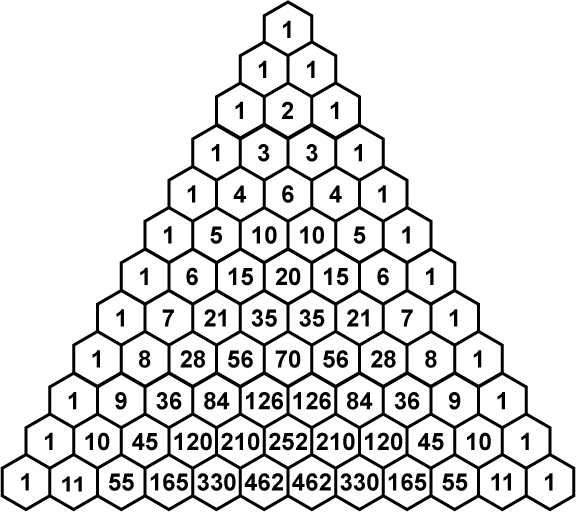
\includegraphics[scale=0.5]{pascal.png}\\
\textit{Pascal's Triangle}
\end{center}
\newpage

%%%%%%%%%%%%%%%%%%%%%%%%%%%%%%%%%%%%%%%%%%%%%%%%%%%%%%%%%%%%%%%%%%%%%%

\section{May 3, 2018}
\subsection{Binomial Theorem}
$(a+b)^{n}$ = $\sum_{k=0}^{n} C_{k}^{n} \cdot a^{k} \cdot b^{n-k}$\\\\
\textbf{Ex 1:} $(a+b)^{3}$ = $C_{0}^{3} \cdot a^{6}b^{3}$ + $C_{1}^{3} \cdot ab^{2}$ + $C_{2}^{3} \cdot a^{2}b$ + $C_{3}^{3} \cdot a^{3}b$ = $b^{3} + 3ab^{2} + 3ba^{3} + a^{3}$\\\\
\textbf{Ex 2:} Find the coefficient of $x^{6}$ in the expansion of $(x^{2}+2)^{7}$.\\
\textbf{Solution:} If we let $x^{2}$ := $a$ and 2 := $b$, then from the binomial theorem:
\[(a+b)^{n} = \sum_{k=0}^{n} C_{k}^{n} \cdot a^{k} \cdot b^{n-k} = \sum_{k=0}^{n} C_{k}^{7} \cdot a^{k} \cdot b^{7-k} = C_{3}^{7} \cdot 2^{4} = 560\]
\subsection{Conditional Probability}
Let $\Om$ be a sample space and let $\bbP$ be a probability on $\Om$. Let $A \subseteq \Om$ be an event such that $\bbP(A)\ \gt\ 0$, and let $B \subseteq \Om$ be another event. The \textit{conditional probability of $B$ given $A$}, is defined as
\[ \bbP(A|B) = \frac{\bbP(B \cap A)}{\bbP(A)}\]\\
$\textbf{Ex 1:}$ We have 2 urns. Urn 1 contains 7 red balls and 4 blue balls, and urn 2 contains 5 red balls and 6 blue balls. First, we choose a ball from urn 1 and place it into urn 2, then we remove a ball from urn 2. What is the probability that the ball that we remove from urn 2 will be blue?\\
\textbf{Solution:} Let $B$ be the event where the ball drawn from urn 2 is blue, and let $A_{r}$, $A_{b}$ be the events where we draw a red or a blue ball from urn 1 respectively. Then $\bbP(A_{r})$ = $\frac{7}{11}$ and $\bbP(A_{b})$ = $\frac{4}{11}$. Also,
\[B = B \cap \Om \iff B = B \cap (A_{r} \cup A_{b}) \iff B = (B \cap A_{r}) \cup (B \cap A_{b})\]
Which then implies
\[\bbP(B) = \bbP(B \cap A_{r}) + \bbP(B \cap A_{b}) \iff \bbP(B) = \bbP(B|A_{r}) \cdot \bbP(A_{r}) + \bbP(B|A_{b}) \cdot \bbP(A_{b})\]
So all that is left is to compute $\bbP(B|A_{r})$, and $\bbP(B|A_{b})$.\\
From the definition, we can see that $\bbP(B|A_{r})$ = $\frac{1}{2}$, and $\bbP(B|A_{b})$ = $\frac{7}{12}$, so finally
\[ \bbP(B) = \frac{6}{12} \cdot \frac{7}{11} + \frac{7}{12} \cdot \frac{4}{11} = \frac{70}{132} \]\\
\textbf{Ex: 2} Roll a fair die. Let $A \subseteq \Om$ be the event where the outcome is even, $B \subseteq \Om$ be the event where the outcome is odd, $C \subseteq \Om$ be the event where the outcome is either a 1 or a 2. Compute all the conditional probabilities.\\
\textbf{Solution} First $\bbP(A) = \frac{1}{2}$, $\bbP(B) = \frac{1}{2}$, and $\bbP(C) = \frac{1}{3}$ Then:\\
$\bbP(A|B) = \frac{\frac{1}{6}}{\frac{1}{2}}$ = $\frac{1}{3}$, and $\bbP(B|A) = \frac{\frac{1}{6}}{\frac{1}{2}}$ = $\frac{1}{3}$\\
$\bbP(A|C) = \frac{1}{2}$, and $\bbP(C|A) = \frac{1}{3}$\\
$\bbP(B|C)$ = 1, and $\bbP(C|B) = \frac{2}{3}$\\
\subsection{Independent Events}
Let $A$, and $B$ be two events over some sample space $\Om$. $A$, and $B$ are said to be $independent$ if and only if:
\begin{enumerate}
	\item $\bbP(A|B)$ = $\bbP(A)$
	\item $\bbP(B|A)$ = $\bbP(B)$
	\item $\bbP(A \cap B)$ = $\bbP(A)$ $\cdot$ $\bbP(B)$
\end{enumerate}
\textbf{Ex: }\\ 
a) From the previous example, are $A$ and $B$ independent? \\
b) What about $A$ and $C$?\\
c) $B$ and $C$?\\
\textbf{Answers:}\\
a) No.\\
b) Yes.\\
c) No.\\
\subsection{Baye's Rule}
Let $A, B \subseteq \Om$ be events on a sample space $\Om$. Then the equation
\[ \bbP(A|B) = \frac{\bbP(B|A) \cdot \bbP(A)}{\bbP(B)}\]
is calles Baye's Rule, or Baye's Theorem.\\\\
\textbf{Theorem:} Total Probability Rule\\ 
Let $\Om$ be a sample space, and let $A \subseteq \Om$ be an event. Suppose we partition $\Om$ like $\Om$ = $\{$$B_{1}, B_{2}, \dots, B_{n}$$\}$, where the $B_{i}$s are pairwise disjoint events such that
\[ \bigcup_{i=1}^{n}B_{i} = \Om\]
Then:
\begin{enumerate}
	\item $\bbP(A)$ = $\sum_{i=1}^{n}$$\bbP(A|B_{i}) \cdot \bbP(B_{i})$, and
	\item If $k \in \N$ is fixed, then $\bbP(B_{k}|A)$ = $\frac{\bbP(A|B_{k}) \cdot \bbP(B_{k})}{\sum_{i=1}^{n}\bbP(A|B_{i}) \cdot \bbP(B_{i})}$
\end{enumerate}
\textbf{Proof:}
\begin{enumerate}
	\item We know that $A$ = $A \cap \Om$ $\iff$ $A$ = $A \cap (\bigcup_{i=1}^{n}B_{i})$ $\iff$ $A$ = $\bigcup_{i=1}^{n}A \cap B_{i}$. Therefore, $\bbP(A)$ = $\sum_{i=1}^{n}\bbP(A \cap B_{i})$ $\iff$ $\bbP(A)$ = $\sum_{i=1}^{n}\bbP(A|B_{i})\cdot \bbP(B_{i})$ \qed
	\item $\bbP(B_{k}|A)$ = $\frac{\bbP(B_{k} \cap A)}{\bbP(A)}$ = $\frac{\bbP(A|B_{k})\cdot \bbP(B_{k})}{\bbP(A)}$ = $\frac{\bbP(A|B_{k}) \cdot \bbP(B_{k})}{\sum_{i=1}^{n}\bbP(A|B_{i}) \cdot \bbP(B_{i})}$ \qed \\\\\\
\end{enumerate}
\textbf{Ex:} A (very simple) forecast model
\\Suppose that on a given day the weather is one of two states: sunny or rainy. Let $R \subseteq \Om$ be the event where it's rainy and $S \subseteq \Om$ be the event where it's sunny. If today is rainy then the probability that tomorrow will also be rainy is 60\%. On the other hand, if today is sunny then the probability that tomorrow will be sunny is 70\%.\\
a) If Monday is sunny then what is the probability that Wednesday will also be sunny?\\
b) If Wednesday is sunny then what is the probability that Tuesday was rainy?\\
\textbf{Solutions:}\\
a) Let $A$ be the event where it is sunny on Wednesday. Then
\[ \bbP(A) = \bbP(A|A_{1}) \cdot \bbP(A_{1}) + \bbP(A|A_{2}) \cdot \bbP(A_{2}) = 0.7 \cdot 0.7 + 0.4 \cdot 0.3 = 0.61\]
where $A_{1}$ is the event where it's sunny on Tuesday, and $A_{2}$ is the event where it's rainy on Tuesday.\\
b) $\bbP(A_{2}|A)$ = $\frac{\bbP(A|A_{2}) \cdot \bbP(A_{2})}{\bbP(A)}$ = $\frac{0.12}{0.61}$ = $\frac{12}{61}$

\newpage

%%%%%%%%%%%%%%%%%%%%%%%%%%%%%%%%%%%%%%%%%%%%%%%%%%%%%%%%%%%%%%%%%%%%%%

\section{May 7, 2018}
\subsection{When to use Permutations vs Combinations}
To determine whether we need to use a permutation or a combination we first need to consider two things. First, the sampling method:
\begin{enumerate}
	\item Without Replacement
	\item With Replacement
\end{enumerate} 
and whether we care about the order of the sample points:
\begin{enumerate}
\setcounter{enumi}{2}
	\item Order doesn't matter
	\item Order matters
\end{enumerate}
We use permutations when we have 1\&4, and\\
we use combinations when we have 1\&3 $or$ 2\&4.
\subsection{Multinomial Coefficients}
The number of ways we can partition $n$ objects into $k$ distinct groups containing $n_{1}$, $n_{n}$, \dots, $n_{k}$ objects, respectively, where each object appears in exactly one group and $\sum_{i=1}^{k} n_{i}$ = $n$, is
\[N := {n\choose{n_{1}, n_{2}, \dots, n_{k}}} = \frac{n!}{n_{1}! n_{2}! \dots n_{k}!} \]
where we call
\[{n\choose{n_{1}, n_{2}, \dots, n_{k}}} \]
the \ti{multinomial coefficient}.\\\\
\textbf{Ex 1:} We wish to expand $(x + y + z)^{17}$. What is the coefficient on the $x^{2}y^{5}z^{10}$ term?\\
\textbf{Solution:} The coefficient is ${17\choose{2, 5, 10}}$ = $\frac{17!}{2!5!10!}$\\\\
\textbf{Ex 2:} \#62 from the first assignment.\\
\textbf{Solution:} Total number = ${9\choose{3, 3, 3}}$, Desired number = ${7\choose{1, 3, 3}}$.\\
Therefore, $\bbP(A)$ = $\frac{{7\choose{1, 3, 3}}}{{9\choose{3, 3, 3}}}$
\subsection{Discrete Random Variables}
\ti{Random Variables} are variables that take on random values based on the outcome of the experiment. Each random variable is associated with a \ti{probability distribution} that specifies the possible random variable values and the probability each value will occur. A random variable is said to be \ti{discrete} if it can get only a finite or countably infinite number of possible distinct values.\\\\
The probability that the random variable $Y$ will take on the value $y$, denoted by $\bbP(Y=y)$, is defined as the sum of the probabilities of all the sample points $\om \in \Om$ that are assigned the value of $y$.
\subsection{Probability Distribution Representations}
The probability distribution for a discrete random variable $Y$ can be represented as a rule (formula), a table, or a graph. \\
\textbf{Ex: }
\begin{center}
\begin{tabular}{| c || c | c | c | c | c | c | c | c | c | c | c |}
\hline
$y$ & 2 & 3 & 4 & 5 & 6 & 7 & 8 & 9 & 10 & 11 & 12\\
\hline
$\bbP(Y=y)$ & $\frac{1}{36}$ & $\frac{2}{36}$ & $\frac{3}{36}$ & $\frac{4}{36}$ & $\frac{5}{36}$ & $\frac{6}{36}$ & $\frac{5}{36}$ & $\frac{4}{36}$ & $\frac{3}{36}$ & $\frac{2}{36}$ & $\frac{1}{36}$\\
\hline
\end{tabular}
\end{center}
is a probability distribution of $y$.\\\\
\underline{Theorem:} For any discrete probability distribution, the following hold:
\begin{enumerate}
	\item $\bbP(Y=y) \geq 0$, $\forall y$
	\item $\sum_{y} \bbP(Y=y)$ = 1
\end{enumerate}
\subsection{Expected Value}
Let $Y$ be a discrete random variable with a probability function $\bbP(Y=y)$. Then the expected value of $Y$, $E(Y)$, is defined to be
\[E(Y) = \sum_{y} y\cdot \bbP(Y=y).\]
The expected value exists only if the above summation is \ti{absolutely convergent}. We often denote $E(Y)$ by $\mu$.\\\\
\textbf{Ex:} Consider a random variable $Y$ with the following probability distribution.
\begin{center}
\begin{tabular}{| c || c | c | c|}
\hline
$y$ & 0 & 1 & 2\\
\hline
$\bbP(Y=y)$ & $\frac{1}{4}$ & $\frac{1}{2}$ & $\frac{1}{4}$\\
\hline
\end{tabular}
\end{center}
Then
\[\mu = \sum_{y} y\cdot \bbP(Y=y) = 0\cdot \frac{1}{4} + 1\cdot \frac{1}{2} + 2\cdot \frac{1}{4} = \frac{1}{2} + \frac{1}{2} = 1\]
\subsection{Expected Value of a Function of a Random Variable}
\underline{Theorem:} Let $Y$ be the discrete random variable with probability function $\bbP(Y=y)$, and let $g(Y)$ be a real-valued function of $Y$. Then, the expected value of $g(Y)$ is
\[E(g(Y)) = \sum_{y} g(Y)\cdot \bbP(Y=y).\]
\subsection{Varience of a Random Variable}
For a random variable $Y$ with mean $E(Y) \equiv \mu$, the \ti{varience} of $Y$, $V(Y)$, is defined as the expected value of $(Y - \mu)^{2}$. That is
\[V(Y) = E((y-\mu)^{2}).\]
The varience represents the "average squared deviation of $Y$ from its mean". Intuitively, it's a measure of how variable a random variable is. The bigger the value of the varience is, the more spread out the values that the random variable can take on are.
\subsection{Standard Deviation of a Random Variable}
The \ti{standard deviation}, $\sigma$, of a random variable $Y$, is defined as the principle square root of $V(Y)$. That is
\[\sigma^{2} = V(Y) \iff \sigma = |\sqrt{V(Y)}|\]
This is a little easier to visualize than varience.
\subsection{Some Theorems (without proof)}
\underline{Theorem:} Let $Y$ be a discrete random variable with the probability function $\bbP(Y=y)$, and let $c \in \R$ be a constant. Then
\[E(c) = c\]
\underline{Theorem:} Let $Y$ be a discrete random variable with the probability function $\bbP(Y=y)$, let $g(Y)$ be a function of $Y$, and let $c$ be a constant. Then
\[E(c\cdot g(Y)) = c\cdot E(g(Y))\]
\underline{Theorem:} Let $Y$ be a discrete random variable with the probability function $\bbP(Y=y)$, and let $g_{1}(Y), g_{2}(Y)$, \dots, $g_{k}(Y)$ be $k$ functions of $Y$. Then
\[E(g_{1}(Y) + g_{2}(Y) + \dots + g_{k}(Y)) = E(g_{1}(Y)) + E(g_{2}(Y)) + \dots + E(g_{k}(Y))\]
\underline{Theorem:} Let $Y$ be a discrete random variable with the probability function $\bbP(Y=y)$ and mean $\mu$. Then
\[V(Y) \equiv \sigma^{2} = E((Y-\mu)^{2}) = E(Y^{2})-\mu^{2}\]
\subsection{Binomial Probability Distribution}
The \ti{binomial probability distribution} is a probability distribution that comes up pretty commonly. It applies where
\begin{itemize}
	\item There's a sequence of independent or identical trials
	\item Each trial can result in one of two outcomes (flipping a coin, for example).
\end{itemize}
More precisely, a binomial experiment is such that
\begin{itemize}
	\item Consists of a fixed number of $n$ trials
	\item Each trial results in one of two possible outcomes: $S$(uccess), or $F$(ailure).
	\item The probability of $S$ on any trial is $p$, and the probability of $F$ on any trial is $q=1-p$.
	\item All trials are independent
	\item The random variable $Y$ is the number of successes out of $n$ trials.
\end{itemize}
A random variable $Y$ is said to have binomial distribution based on $n$ trials iff
\[\bbP(Y=y) = {n\choose{y}}p^{n}q^{n-y}\]

\newpage

%%%%%%%%%%%%%%%%%%%%%%%%%%%%%%%%%%%%%%%%%%%%%%%%%%%%%%%%%%%%%%%%%%%%%%

\section{May 8, 2018}
\subsection{Bernoulli Distribution}
Let $X$ be a random variable. Toss a coin. The outcomes are $H$, and $T$. Set $X(H) = 1$, and $X(T) = 0$. We have $X(\Om) = \{0, 1\}$.\\ Assume $\bbP(H) = p$, for $0\ \lt\ p\ \lt\ 1$. Then the probability function $\bbP(X=x)$ of $X$ is
\begin{center}
\begin{tabular}{| c || c | c |}
\hline
$x$ & 0 & 1\\
\hline
$\bbP(X = x)$ & 1-p & p\\
\hline
\end{tabular}
\end{center}
A random variable $X$ that has the above probability function is called a \ti{Bernoulli random variable} on $X$. Also, $X$ is said to have the \ti{Bernoulli Distribution} with parameter $p$. We write $X \sim$ Ber($p$).\\\\
\underline{Proposition:} If $X \sim$ Ber($p$), then
\begin{enumerate}
	\item $E(X) = p$
	\item $V(X) = p(1-p)$
\end{enumerate}
\underline{Proof} of (1):\\
$E(X) = \sum_{x} x\cdot \bbP(X=x)$\ = $0\cdot \bbP(X=0) + 1\cdot \bbP(X=1) = p.$ \qed \\\\
\underline{Proof} of (2):\\
$V(X) = E(X-E(X)^{2})$ = $E(X^{2}) - (E(X))^{2}$.\\
Also, $E(X^{2})$ = $\sum_{x} x^{2}\cdot \bbP(X=x)$ = $p$.\\
Therefore, $V(X) = p-p^{2} = p(1-p)$. \qed
\subsection{Some Properties of $E$, and $V$}
Let $X$ be a random variable, and let $c, \alpha \in \R$ be constants.
\begin{enumerate}
	\item $E(X+c)=E(X)+c$
	\item $V(X+c)=V(X)$
	\item $E(\alpha X)=\alpha E(X)$
	\item $V(\alpha X)=\alpha^{2} V(X)$
\end{enumerate}
\ \\\\
\subsection{A Proof that $V(X) = E(X^{2}) - (E(X))^{2}$}
Property: If $f$, $g$ are functions, then $E(f(x) + g(x)) = E(f(x)) + E(g(x))$.\\\\
Set $\mu := E(X)$. Then, by definition,
\begin{align*}
	V(X) &= E((X-E(X))^{2})\\
		&= E(x^{2} -2\mu x + \mu^{2})\\
		&= E(X^{2}) -2\mu E(X) + \mu^{2}\\
		&= E(X^{2})-2\mu^{2} + \mu^{2}\\
		&= E(X^{2}) - \mu^{2}\\
		&= E(X^{2}) - (E(X))^{2}
\end{align*}
\qed
\subsection{More on Binomial Distribution}
\underline{Proposition:} If $X \sim$ Bin($n$, $p$), then
\begin{enumerate}
	\item $E(X) = np$
	\item $V(X) = np(1-p)$
\end{enumerate}
To prove there we first have to note that
\[k\cdot {n\choose k} = k\cdot \frac{n!}{k!(n-k)!} = n\cdot \frac{(n-1)!}{(k-1)!(n-k)!} = n\cdot {{n-1}\choose{k-1}}\]\\
\underline{Proof} of (1): By definition,
\begin{align*}
	E(X) &= \sum_{k=0}^{n} k\cdot \bbP(X=k)\\
		&= \sum_{k=0}^{n} k\cdot {n\choose k}\cdot p^{k}(1-p)^{n-k}\\
		&= \sum_{k=0}^{n} n\cdot {{n-1}\choose{k-1}}\cdot p^{k}(1-p)^{n-k}\\
		\intertext{Let $\ell = k-1$}
		&= n\cdot \sum_{\ell = 0}^{n-1} {{n-1}\choose{\ell}}\cdot p^{\ell + 1}(1-p)^{(n-1)-\ell}\\
		&= np\cdot \sum_{\ell=0}^{n-1} {{n-1}\choose{\ell}}\cdot p^{\ell}(1-p)^{(n-1)-\ell}\\
		&= np(p+(1-p))^{n-1}\\
		&= np
\end{align*}
\qed\\\\
\underline{Proof} of (2): By definition, 
\begin{align*}
	V(X) &= E(X^{2}) - n^{2}p^{2}\\
		&= E(X(X-1)+X) - n^{2}p^{2}\\
		&= E(X(X-1))+np-n^{2}p^{2}\\
\end{align*}
Now we need to reduce $E(X(X-1))$  down.
\begin{align*}
	E(X(X-1)) &= \sum_{k=0}^{n} k\cdot (k-1)\cdot {n\choose k}\cdot p^{k}(1-p)^{n-k}\\
			&= \sum_{k=2}^{n} k\cdot (k-1)\cdot {n\choose k}\cdot p^{k}(1-p)^{n-k}
\end{align*}
Now we need to change the variables in $k(k-1)\cdot {n\choose k}$.
\[k\cdot (k-1)\cdot {n\choose k} = n\cdot (n-1)\cdot {{n-2}\choose{k-2}}\]
so now plugging that back into $E(X)$ we get
\begin{align*}
	E(X(X-1)) &= \sum_{k=2}^{n} k\cdot (k-1)\cdot {n\choose k}\cdot p^{k}(1-p)^{n-k}\\
			&= \sum_{k=2}^{n} n\cdot (n-1)\cdot {{n-2}\choose{k-2}}\cdot p^{k}(1-p)^{n-k}
			\intertext{Let $\ell = k-2$}
			&= n\cdot (n-1)\cdot \sum_{\ell =0}^{n-2} {{n-2}\choose{\ell}}\cdot p^{\ell}(1-p)^{(n-2)-\ell}\\
			&= n\cdot(n-1)\cdot p^{2}\cdot (p + (1-p))^{n-2}\\
			&= n\cdot(n-1)\cdot p^{2}
\end{align*}
Plugging this back into $V(X)$, we get
\begin{align*}
	V(X) &= E(X(X-1))+np-n^{2}p^{2}\\
		&= n\cdot(n-1)\cdot p^{2} + np - n^{2}p^{2}\\
		&= np -np^{2}\\
		&= np(1-p)
\end{align*}
\qed\\\\
\textbf{Ex 1:} 3.60 from the textbook\\\\
\textbf{Solution} Fish die with $\bbP$ = 0.2. Therefore the prob of a success (they survive), $\bbP(S)$ = 0.8. Let the random variable $X$ be the number of fish that survive. There are 20 fish. Thus $X \sim$ Bin($n=20$, $p=0.8$). The probability that 14 fish survive is
\[\bbP(X=14) = {20\choose 14}\cdot (0.8)^{14}\cdot(0.2)^{6} \approx 0.1091 = 10.91\%\]
\subsection{Geometric Distribution}
FIrst recall that
\[\sum_{n=0}^{\infty} x^{n} = \frac{1}{1-x}, \  |x|\ \lt\ 1.\]\\
Suppose an experiment leads to either an $S(uccess)$ or an $F(ailure)$. Suppose we want to repeat the experiment until an $S$ occurs\\
Let $\bbP(S) = p$, when 0 \lt $p$ \lt 1, and of course, $\bbP(F) = 1-p$. Then
\[\Om = \{\om_{1}, \om_{2}, \dots, \om_{n}\}\]
where 
\[\om_{n} = FFF\dots FS\]
with $n-1\ Fs$.\\
Let the random variable $X$ reperesent the number of trials needed for as $S$ to occur. Then
\[\Om(X) = \N\]
The probability function of $X$ is then
\[\bbP(X=k) = p\cdot (1-p)^{k-1}\]
If $X$ satisfies this then we write $X \sim$ Geometric($p$).\\\\
\underline{Proposition:}
\begin{enumerate}
	\item $E(X) = \frac{1}{p}$
	\item $V(X) = \frac{1}{p}\cdot (\frac{1}{p} - 1)$
\end{enumerate}
\underline{Proof} of (1): By definition
\begin{align*}
	E(X) &= \sum_{k=1}^{\infty} k\cdot \bbP(X=k)\\
		&= \sum_{k=1}^{\infty} k\cdot p\cdot (1-p)^{k-1}\\
		&= p\cdot \sum_{k=1}^{\infty} k\cdot (1-p)^{k-1}\\
		&= p\cdot \frac{1}{(1-(1-p))^{2}}\\
		&= \frac{p}{p^{2}}\\
		&= \frac{1}{p}
\end{align*}
\qed\\
\underline{Proof} of (2): By definition
\begin{align*}
	V(X) &= E(X^2) - (E(X))^2\\
		&= E(X^2) - \frac{1}{p^2}\\
		&= E(X(X-1)) + E(X) - \frac{1}{p^2}\\
		&= E(X(X-1)) + \frac{1}{p} - \frac{1}{p^2}
\end{align*}
Now we need to reduce down $E(X(X-1))$
\begin{align*}
	E(X(X-1)) &= \sum_{k=1}^{\infty} k\cdot p\cdot (k-1)\cdot (1-p)^{k-1}\\
			&= p\cdot (1-p)\cdot \sum_{k=2}^{\infty} k\cdot (k-1)(1-p)^{k-2}\\
			&= p\x (1-p)\x \frac{2}{p^{3}}\\
			&= \frac{2(1-p)}{p^2}
\end{align*}
Plugging this back into $V(X)$, we get
\begin{align*}
	V(X) &= E(X(X-1)) + \frac{1}{p} - \frac{1}{p^2}\\
		&= \frac{2(1-p)}{p^2} + \frac{1}{p} - \frac{1}{p^2}\\
		&= \frac{2 -2p +1 -1}{p^2}\\
		&= \frac{1-p}{p^2}\\
		&=\frac{1}{p}\x \Big(\frac{1}{p} -1\Big)
\end{align*}
\qed
\newpage

%%%%%%%%%%%%%%%%%%%%%%%%%%%%%%%%%%%%%%%%%%%%%%%%%%%%%%%%%%%%%%%%%%%%%%

\section{May 9, 2018}
\subsection{Hypergeometric Distribution}
Suppose we have a population of size $N$, and a subpopulation of size $r$. Each member of the subpopulation has a certain characteristic that the remaining $N - r$ members do not have. Take a sample from the population of size $n$. Then, let $X$ be the random variable containing the number of elements from the subpopulation in the sample.\\\\
\textbf{Ex:} Suppose we draw a 5-card hand out of a deck of 52 cards . Let $X$ be the number of aces in the hand. What are the possible values that $X$ can take on?\\
\textbf{Solution:} We have $N=52$, $n=5$, and $r=4$, and we want to find $X(\Om)$.\\
First, $X \leq n$, and $X \leq r$ $\imply$ $X\leq$ min\{$n, r$\}.\\
Also $n - X \leq n$, and $n-X \leq N-r$ $\imply$ $X \geq 0$, and $X \geq n+r-N$, and therefore $X \geq$ max\{$0, n+r-N$\}.\\
So, $X \in \Z$ such that
\begin{center}
max\{$0, n+r-N$\} $\leq X \leq$ min\{$n, r$\}\\
$\imply$ max\{$0, 9-52$\} $\leq X \leq$ min\{$4, 5$\}\\
$\imply$ 0 $\leq X \leq$ 4
\end{center}
And thus $X \in$ \{0, 1, 2, 3, 4\}, which makes sense.\\\\
\underline{Theorem:} Suppose $X$ is a hypergeometric distribution with parameters $N$, $n$, and $r$. Then
\begin{enumerate}
	\item $E(X) = n\x \frac{r}{N}$
	\item $V(X) = (n\x \frac{r}{N})(1 - \frac{r}{n})(\frac{N-n}{N-1})$
\end{enumerate}
We will prove this later when we're on chapter 5.
\subsubsection{The Probability Function of X}
If $k \in \N_{0}$ such that max\{$0, n+r-N$\} $\leq k \leq$ min\{n, r\}, then
\[p_{X}(k) = \bbP(X=k) = \frac{C_{k}^{r}\x C_{n-k}^{N-r}}{C_{n}^{N}}\]
A random variable $X$ with the above probability function is calles a \ti{hypergeometric distribution} with parameters $N$, $n$, and $r$, and we write 
\begin{center}
$X \sim$ Hypergeometric($N$, $n$, $r$).
\end{center}
\textbf{Ex:} Let $X$ be the number of aces in a 5-card hand drawn from a 52-card deck. Then
\begin{align*}
	p_X(0) &= \frac{C_{0}^{4}\x C_{5}^{48}}{C_{5}^{52}}\\
	p_X(1) &= \frac{C_{1}^{4}\x C_{4}^{48}}{C_{5}^{52}}\\
	p_X(2) &= \frac{C_{2}^{4}\x C_{3}^{48}}{C_{5}^{52}}\\
	\vdots
\end{align*}
\subsection{Poisson Distribution}
Recall if $\la \in \R$ then
\[e^{\la} = \sum_{n=0}^{\infty} \frac{\la^{n}}{n!}\]
Let $\la \geq 0$ be fixed. The function
\[p(n) = e^{-\la}\x \frac{\la^{n}}{n!}\]
for $n \in\N$ is a probability function. This isn't immediately obvious and requires proof.\\
Proof:
\begin{align*}
	\sum_{n=0}^{\infty} p(n) &= e^{-\la}\x \sum_{n=0}^{\infty} \frac{\la^{n}}{n!}\\
						&= e^{-\la}e^{\la}\\
						&= 1
\end{align*}
\qed\\
A random variable $X$ with the above probability function is said to have \ti{poisson distribution} with parameter $\la$. We write $X \sim$ Poisson($\la$).\\\\
\underline{Proposition:} Assume $X \sim$ Poisson($\la$). Then
\begin{enumerate}
	\item $E(X) = \la$
	\item $V(X) = \la$
\end{enumerate}
\underline{Proof} of (1): By definition
\begin{align*}
	E(X) &= \sum_{n=0}^{\infty} n\x p_{x}(n)\\
		&= \sum_{n=1}^{\infty} n\x e^{-\la}\x \frac{\la^{n}}{n!}\\
		&= e^{-\la}\x \sum_{n=1}^{\infty} \frac{\la^{n}}{(n-1)!}\\
		&= \la\x e^{-\la}\x \sum_{n=1}^{\infty} \frac{\la^{n-1}}{(n-1)!}\\
		&= \la\x e^{-\la}\x \sum_{n=0}^{\infty} \frac{\la^{n}}{n!}\\
		&= \la\x e^{-\la}\x e^{\la}\\
		&= \la
\end{align*}
\qed\\
\underline{Proof} of (2): By definition
\begin{align*}
	V(X) &= E(X^{2}) - (E(X))^{2}\\
		&= E(X(X-1)) + E(X) - (E(X))^{2}\\
		&= E(X(X-1)) + \la - \la^{2}\\
		&= \sum_{n=2}^{\infty}[n(n-1)\x p_{X}(n)] +\la - \la^{2}\\
		&= \la^{2} e^{-\la}\x \sum_{n=2}^{\infty} \bigg[\frac{\la^{n-2}}{(n-2)!}\bigg] +\la - \la^{2}\\
		&= \la^{2} e^{-\la}\x \sum_{n=0}^{\infty} \bigg[\frac{\la^{n}}{n!}\bigg] +\la - \la^{2}\\
		&= \la^{2} e^{-\la} e^{\la} +\la - \la^{2}\\
		&= \la^{2} +\la - \la^{2}\\
		&= \la
\end{align*}
\qed\\\\
\textbf{Ex 1:} 3.122 from the book.\\
\textbf{Solution:} Let $X$ be the number of customers at a store. 7 is the mean $\imply$ \\$X \sim$ Poisson($\la =7$).\\
a) $\bbP(X\leq 3)$ = $\sum_{n=0}^{3} p_{X}(n)$ = $\sum_{n=0}^{3} e^{-7}\x \frac{7^{n}}{n!}$\\
b) $\bbP(X\geq 2)$ = $1-\bbP(x\ \lt\ 2) = 1-\bbP(x\leq 1)$ \dots\ plug into probability function. \\\\
\textbf{Ex 2:} Assume that $X_{1} \sim$ Poisson($\la_{1}$), $X_{2} \sim$ Poisson($\la_{2}$). Suppose $X_{1}$, $X_{2}$ are independent events, and \{$X_{1} = n_{1}$\}, \{$X_{2} = n_{2}$\} are independent events for every $n_{1}$, $n_{2}$, $\in \N$. Prove that the distribution given by $X = X_{1} + X_{2}$ is also poisson.\\
\textbf{Solution:} Proceeding by induction on $n$, we have\\
\underline{Base Case:} $n=1$
\begin{align*}
	\bbP(X=1) &= \bbP((X_{1} = 1 \wedge X_{2} = 0)\vee (X_{1} = 0 \wedge X_{2} = 1))\\
			&= \bbP(X_{1} = 1 \wedge X_{2} = 0) + \bbP(X_{1} = 0 \wedge X_{2} = 1)\\
			&= \bbP(X_{1} = 1) \bbP(X_{2} = 0) + \bbP(X_{1} = 0) \bbP(X_{2} = 1)\\
			&= \la_{1}e^{-\la_{1}}e^{-\la_{2}} + \la_{2}e^{-\la_{1}}e^{-\la_{2}}\\
			&= (\la_{1} + \la_{2})e^{-(\la_{1} + \la{2})}
\end{align*}
\begin{flushright}
Q.E.D
\end{flushright}
\underline{Inductive Step:} $n=k$
\begin{align*}
	\bbP(X=k) &= \sum_{i=0}^{k} \bbP(X_{1}=i\ \wedge\ X_{2}=k-i)\\
			&= \sum_{i=0}^{k} \bbP(X_{1}=i)\bbP(X_{2}=k-i)\\
			&= e^{-(\la_{1} + \la_{2})}\x \sum_{i=0}^{k} \frac{\la_{1}^{i}}{i!}\x \frac{\la_{2}^{k-i}}{(k-i)!}\\
			&= \frac{e^{-(\la_{1}+\la_{2})}}{k!}\x \sum_{i=0}^{k} \frac{k!}{i!(k-i)!} \la_{1}^{i}\la_{2}^{k-i}\\
			&= \frac{e^{-(\la_{1}+\la_{2})}}{k!}\x \sum_{i=0}^{k} {k\choose i} \la_{1}^{i}\la_{2}^{k-i}\\
			&= \frac{e^{-(\la_{1}+\la_{2})}}{k!}(\la_{1}+\la_{2})^{k}
\end{align*}
\begin{flushright}
Q.E.D
\end{flushright}
And thus by induction, the distribution of the random variable, formed by summing two random variables with poisson distribution, is itself poisson.\\
\qed\\\\\\
\subsection{Moment Generating Functions}
First we will define \ti{moments of a random variable}. Let $X$ be a random variable. The $n^{th}$ moment of $X$, $\mu_{n}$, is defined as
\[\mu_{n} = E(X^{n})\]
for $n \in \N$.\\\\
\underline{Remark:} If $X$ is  a discrere random variable, then
\[\mu_{n} = E(X^{n}) = \sum_{x} x^{n}\x p_{X}(x)\]\\
Now we'll define \ti{moment generating functions (MGFs)}. Let $X$ be a random variable. The moment generate function of $X$ is defined as
\[m_{X}(t) = E(e^{tX})\]
\underline{Remark:}
\begin{enumerate}
	\item $t=0$ is always in the domain of $m_{X}$
	\item The moment generating function, $m_{X}$, of $X$ is a unique identification of the distribution of $X$, not unlike Laplace transforms serve as a unique identification for differential equation solutions!
\end{enumerate}
\ \\
\textbf{Ex 1:} Consider the probability distribution given by
\begin{center}
\begin{tabular}{| c || c | c | c |}
\hline
$x$ & 0 & -1 & 3\\
\hline
$\bbP(X=x)$ & $\frac{1}{4}$ & $\frac{1}{2}$ &  $\frac{1}{4}$\\
\hline
\end{tabular}
\end{center}
find the moment generating function.\\
\textbf{Solution:} Straight from the definition of the moment generating function, we have
\begin{align*}
	m_{x}(t) &= E(e^{tX}) = \sum_{x} x^{n}\x p_{X}(x)\\
			&= e^{0t}\x p_{X}(0) + e^{-t}\x p_{X}(-1) + e^{3t}\x p_{X}(3)\\
			&= \frac{1}{4}(1+e^{3t}) + \frac{1}{2}e^{-t},\ t \in \R
\end{align*}
\ \\
\textbf{Ex 2:} Let $X$ be a random variable. Consider the moment generating function of $X$, $m_{X}(t)$ given by
\[m_{X}(t) = \frac{1}{2}e^{t} + \frac{1}{6}e^{5t} + \frac{1}{3}e^{-6t}\]
write the probability distribution.\\\\\\
\textbf{Solution:}\\
\begin{center}
\begin{tabular}{| c || c | c | c |}
\hline
$x$ & 1 & 5 & 6\\
\hline
$\bbP(X=x)$ & $\frac{1}{2}$ & $\frac{1}{6}$ & $\frac{1}{3}$\\
\hline
\end{tabular}
\end{center}
It's pretty easy to see the relationship between the equatoin and the table.\\\\
\underline{Remark:}
\begin{align*}
	m_{X}(t) &= E(e^{tX})\\
			&= E\Bigg(\sum_{n=0}^{\infty} \frac{(tX)^{n}}{n!}\Bigg)\\
			&= \sum_{n=0}^{\infty} E\bigg(\frac{(tX)^{n}}{n!}\bigg)\\
			\intertext{(Of course one needs to be careful of doing the last step!)}
	m_{X}(t) &=  \sum_{n=0}^{\infty} \frac{E(X^{x})}{n!}t^{n}
\end{align*}
If that holds on an interval of the form ]$-\ep, \ep$[, then
\[\frac{d^{n}}{dt^{n}}(m_{X}(t)) \bigg\rvert_{t=0} = E(X^{n})\]
We can write this more formally as a theorem.\\\\
\underline{Theorem:} Let $\ep\ \gt\ 0$, and let $X$ be a random variable such that the moment generating function contains an interval of the form ]$-\ep, \ep$[. Then
\[E(X^{n}) = \frac{d^{n}}{dt^{n}}(m_{X}(t))\bigg\rvert_{t=0}\]
We will not prove this right now. ..Maybe later.\\\\\\\\\\
\subsection{The MGF of the Binomial Distribution}
\underline{Proposition:} Let $X$ be a random variable and suppose that $X \sim$ Bin($n, p$). Then
\[m_{X}(t) = (pe^{t} + (1-p))^{n}\]
for $t \in \R$.\\
\underline{Proof:} By definition, we have
\begin{align*}
	m_{X}(t) &= \sum_{k=0}^{n} e^{tk}\x p_{X}(n)\\
	\intertext{Substituting in the probability function for the binomial distribution, we get}
			&= \sum_{k=0}^{n} {n\choose k} e^{tk}p^{k}(1-p)^{n-k}\\
			&= \sum_{k=0}^{n} {n\choose k} (pe^{t})^{k}(1-p)^{n-k}\\
			&= (pe^{t} + (1-p))^{n}, \ t\in \R
\end{align*}
\qed \\\\
\underline{Proposition:} Let $X$ be a random variable and suppose that $X \sim$ Bin($n, p$). Then
\[E(X) = np\]
\underline{Proof:} 
\begin{align*}
	E(X^{n}) &= \frac{d^{n}}{dt^{n}}(m_{X}(t))\bigg\rvert_{t=0}\\
	\intertext{Setting $n=1$}
	E(X) &= \frac{d}{dt}(m_{X}(t))\bigg\rvert_{t=0}\\
		&= \frac{d}{dt}\big[(pe^{t} + (1-p))^{n}\big] \Big\rvert_{t=0}\\
		&= np(pe^{t} + (1-p))^{n-1}\x e^{t} \Big\rvert_{t=0}\\
		&= np
\end{align*}
\qed\\
Note that finding $V(X)$ is just a matter of finding $\frac{d^{2}}{dt^{2}}$.
\newpage

%%%%%%%%%%%%%%%%%%%%%%%%%%%%%%%%%%%%%%%%%%%%%%%%%%%%%%%%%%%%%%%%%%%%%%

\section{May 10, 2018}
\subsection{The MGF of the Geometric Distribution}
\underline{Proposition:} Let $X$ be a random variable and suppose that $X \sim$ Geometric($p$). Then
\[m_{X}(t) = \frac{pe^{t}}{1-(1-p)e^{t}}, \ t\ \lt\ \ln\bigg(\frac{1}{1-p}\bigg)\]
\underline{Proof:}
\begin{align*}
	m_{X}(t) = E(e^{tX}) &= \sum_{n=1}^{\infty} e^{nt}p_{X}(n)\\
					&= \sum_{n=1}^{\infty} e^{nt}(1-p)^{n-1}p\\
					&= pe^{t}\x \sum_{n=1}^{\infty} ((1-p)e^{t})^{n-1}\\
					&= pe^{t}\x \sum_{n=0}^{\infty} ((1-p)e^{t})^{n}\\
					 &= \frac{pe^{t}}{1-(1-p)e^{t}}, \ t\ \lt\ \ln\bigg(\frac{1}{1-p}\bigg)
\end{align*}
\qed
\subsection{The MGF of the Poisson Distribution}
\underline{Proposition:} Let $X$ be a random variable, let $\la\ \gt\ 0$, and suppose that\\ $X \sim$ Poisson($\la$). Then
\[m_{X}(t) = e^{\la(e^{t}-1)}\]
\underline{Proof:}
\begin{align*}
	m_{X}(t) = E(e^{tX}) &= \sum_{n=0}^{\infty} e^{nt}p_{X}(n)\\
					&= \sum_{n=0}^{\infty} e^{nt}e^{-\la}\x \frac{\la^{n}}{n!}\\
					&= e^{-\la}\x \sum_{n-0}^{\infty}\frac{(\la e)^{n}}{n!}\\
					&= e^{-\la}e^{\la e^{t}},\ \forall\ t \in \R\\
			m_{X}(t) &= e^{\la(e^{t}-1)},\ t \in \R
\end{align*}
\qed\\\\
\textbf{Ex:} Let $X$ be the random variable containing the number of defects in a fabric. Suppose $X \sim$ Poisson($\la=4$). The company pays a cost C of $C := 3^{X}$ for each defect. Find the expected cost.\\
\textbf{Solution:} We want to find $E(3^{X})$.
\begin{align*}
	E(3^{X}) &= m_{X}(t=\ln(3))\\
			&= e^{4(e^{\ln{3}}-1)}\\
			&= e^{4\x 2}\\
			&= e^{8}
\end{align*}
\subsection{Chebyshev's Inequality}
\underline{Theorem:} Let $X$ be a random variable, let $E(X) := \mu$, and let $V(X) := \sigma^{2}$. Then
\[\bbP(|x-\mu|\ \geq\ k\sigma)\ \leq\ \frac{1}{k^{2}}\]
\underline{Lemma:} (*) If $X_{1}$, $X_{2}$ are random variables with $X_{1}\ \geq\  X_{2}$, then
\[E(X_{1}) \geq E(X_{2})\]
\underline{Proof of (*):} We will prove this in chapter 5.\\\\
\underline{Proof:} Let $Y$ be an arbitrary random variable such that $E(Y) = 0$, and such that $V(Y) = 0$. Let $k \in \R$ be fixed. We want to show that
\[\bbP(|Y|\ \geq\ k\sigma)\ \leq\ \frac{1}{k^{2}}\]
Let $Z$ be a random variable such that:
\[Z :=
\begin{cases}
	1, &\text{if}\ |Y|\ \geq\ k\sigma\\
	0, &\text{otherwise}
\end{cases}\]
Therefore
\begin{align*}
	&\ \ \ \ \ |Y|\ \geq\ (k\sigma)\x Z\\
	&\imply |Y|^{2}\ \geq\ (k^{2}\sigma^{2})\x Z^{2}\\
	&\imply |Y|^{2}\ \geq\ (k^{2}\sigma^{2})\x Z\\
	&\imply E(Y^{2})\ \geq\ E((k^{2}\sigma^{2})\x Z)\\
	&\imply E(Y^{2})\ \geq\ k^{2}\sigma^{2}\x E(Z)\\
	&\imply E(Y^{2})\ \geq\ k^{2}\sigma^{2}\x \bbP(|Y|\ \geq\ k\sigma)\\
	&\imply \frac{E(Y^{2})}{k^{2}\sigma^{2}}\ \geq\ \bbP(|Y|\ \geq\ k\sigma)\\
	&\imply \frac{1}{k^{2}}\ \geq\ \bbP(|Y|\ \geq\ k\sigma)\\
\end{align*}
Since $Y$ was arbitrary, we conclude that if we set $Y := X-\mu$, then we have
\[\bbP(|X-\mu|\ \geq\ k\sigma)\ \leq \frac{1}{k^{2}}\]
\qed
\subsection{The Cumulative Distribution Function}
The \ti{Cumulative Distribution Function}. Let $X$ be a random variable. The cuumulative distribution function (cdf) is defined as
\[F_{X}(x) = \bbP(X \leq x)\]\\
\textbf{Ex:} Let $X$ be a discrete random variable whose probability function is given by the table
\begin{center}
\begin{tabular}{| c || c | c | c |}
\hline
$x$ & -1 & 0 & 2\\
\hline
$\bbP(X=x)$ & $\frac{1}{2}$ & $\frac{1}{3}$ & $\frac{1}{6}$\\
\hline
\end{tabular}
\end{center} 
This gives us the cumulative distribution function $F_{X}(x)$
\[ F_{X}(x) =
\begin{cases}
	0, &\text{if}\ x\ \lt\ -1\\
	\frac{1}{2}, &\text{if}\ -1\ \leq\ x\ \lt\ 0\\
	\frac{5}{6}, &\text{if}\ 0\ \leq\ x\ \lt\ 2\\
	\frac{1}{2}, &\text{if}\ x\ \geq\ 2\\
\end{cases}
\]
Note that in this case $F_{X}(x)$ is a right-continuous nondecreasing step-function, such that $\lim_{x\to-\infty} F_{X}(x) = 0$, and $\lim_{x\to\infty} F_{X}(x) = 1$.
\subsection{Continuous Random Variables}
A random variable $X$ is said to be \ti{continuous} if its cumulative distribution function $F_{X}(x)$ is a continuously nondecreasing function such that $\lim_{x\to-\infty} F_{X}(x) = 0$, and $\lim_{x\to\infty} F_{X}(x) = 1$.
\subsection{Computing Probability with the Cumulative Distribution Function}
$\bbP(a \leq X \leq b) = \bbP(X \leq b) - \bbP(X \lt a)$.\\
Note that $\bbP(X=a) = 0 \imply \bbP(X\lt a) = \bbP(X\leq a) = F_{X}(a)$, where $F_{X}$ is the cumulative distribution function of a random variable $X$, so
\begin{align*}
	\bbP(a \leq X \leq b) &= F_{X}(b) - F_{X}(a)\\
					&= \bbP(a \leq X \lt b)\\
					&= \bbP(a \lt X \leq b)\\
					&= \bbP(a \lt X \lt b)
\end{align*}
Note that $\bbP(X \geq a) = \bbP(X \gt a) = 1-F_{X}(a)$\\\\
\textbf{Ex 1:} Let $X$ be a random variable, and let
\[F_{X}(x) = \frac{2}{\pi}\Big(\tan^{-1}(x) + \frac{\pi}{2}\Big)\]
In this case, $F_{X}(x)$ is not a cumulative distribution function because $\lim{x\to\infty} = 2$. However
\[F_{X}(x) = \frac{1}{\pi}\Big(\tan^{-1}(x) + \frac{\pi}{2}\Big)\] indeed is a cumulative distribution function.\\\\
In the above example, the random variable $X$ for which $F_{X}$ is a cumulative distribution function, is said to have the \ti{Cauchy distribution}.\\\\
\textbf{Ex 2:} Let $X$ be a random variable with the Cauchy distribution.\\
Find $\bbP(X \geq 1)$, and $\bbP(-1 \leq X \leq 1)$.\\
\textbf{Solution:} To find $\bbP(X \geq 1)$ we do
\[\bbP(X \geq 1) = 1-F_{X}(1) = 1-\frac{3}{4} = \frac{1}{4}\]
and to find $\bbP(-1 \leq X \leq 1)$ we do
\[\bbP(-1 \leq X \leq 1) = F_{X}(1) - F_{X}(-1) = \frac{1}{2}\]\\
\underline{Theorem:} If $F$ is a cumulative distribution function, then $F$ is differentiable almost everywhere.\\
\underline{Proof:} Take honours analysis 4 lol.
\subsection{Probability Density Function}
Let $F$ be a cumulative distribution function, let $X$ be a random variable, and let $f : \R \to \R$ be a function such that $f(x) = F'(x)$. Then if, $f(x) \geq 0$, and $\int_{-\infty}^{\infty} f(x)\ dx=1$, then $f$ is called a \ti{probability density function} of $X$. The cumulative distribution function of $X$ is given by $F_{X}(x) = \int_{-\infty}^{x} f(t)\ dt$.\\\\
\textbf{Ex 1:} The Cauchy distribution
\[F_{X}(x) = \frac{1}{\pi}\Big(\tan^{-1}(x) + \frac{\pi}{2}\Big)\]
has a probability density function given by
\[f(x) = F'_{x}(x) = \frac{1}{\pi}\x \frac{1}{1 + x^2}, \ \forall\ x \in \R\]\\
\textbf{Ex 2:} Consider the function $f : \R \to \R$ given by
\[f(x) =
\begin{cases}
	cx^{2}e^{-2x}, &\text{if}\ x\ \gt\ 0\\
	0, &\text{otherwise}
\end{cases}\]
Find $c$ such that $f$ is a probability density function.\\
\textbf{Solution:} If $f$ is a probability density function, then $c$ is such that
\begin{align*}
c\int_{0}^{\infty} x^{2}e^{-2x}\ dx &= 1
\intertext{which implies that}
							c &= \frac{1}{\int_{0}^{\infty} x^{2}e^{-2x}\ dx}
\end{align*}
\newpage

%%%%%%%%%%%%%%%%%%%%%%%%%%%%%%%%%%%%%%%%%%%%%%%%%%%%%%%%%%%%%%%%%%%%%%

\section{May 14, 2018}
\subsection{More on CDFs and PDFs}
Suppose $X$ is a continuous random variable. The distribution of $X$ is defined by either its cumulative distribution function $F_{X}$ or its probability density function $f_{X}$, where of course the relationship between the two is
\[F'_{X} = f_{X}\]
We define the \ti{support of the distribution}  to be the set
\[\{x\in \R : f_{X}(x)\ \gt\ 0\}\]
\textbf{Ex:} Consider the CDF
\[
f_{X}(x) =
\begin{cases}
	1, &\text{if}\ x \in\ ]0, 1[\\
	0, &\text{otherwise}
\end{cases}
\]
Then $f_{X}(x) \geq 0$, the support of the distribution is the interval ]0, 1[, and
\[\int_{-\infty}^{\infty}f_{X}(x)\ dx = \int_{0}^{1} f_{X}(x)\ dx = 1\]\\
\textbf{Proposition:} Let $X$ be a continuous random variable and $f_{X}$ be its PDF. Set $Y := aX + b$, $a \neq 0$. Then, the PDF of $Y$ is
\[f_{Y}(y) = \frac{1}{|a|}f_{X}\bigg(\frac{y-b}{a}\bigg)\]
\textbf{Proof:} Let $F_{X}$ be the CDF of $X$. The CDF of $Y$ is then
\[F_{Y}(y) = \bbP(Y\leq y) = \bbP(aX + b \leq y) = \bbP\bigg(X \leq \frac{y-b}{a}\bigg) = F_{X}\bigg(\frac{y-b}{a}\bigg)\]
The PDY of $Y$ is thus
\[f_{Y}(y) = F'_{Y}(y) = \frac{1}{a} f_{X}\bigg(\frac{y-b}{a}\bigg)\]
\qed
\subsection{Expected Value of a Continuous Random Variable}
Let $X$ be a continuous random variable and $f_{X}(x)$ be its PDF. If $g : \R \to \R$ is a function, then
\[E(g(x)) = \int_{-\infty}^{\infty}g(x)f_{X}(x)\ dx\]
if and only if the integral converges. In particular, as in the discrete case
\[E(X) = \int_{-\infty}^{\infty} xf_{X}(x)\ dx\]
\subsection{Variance of a Continuous Random Variable}
Let $\mu := E(X)$. Much like with discrete random varibales, we define the variance of a function, $V(X)$, as
\[V(X) = E((X-\mu)^{2})\]
in particular
\[V(X) = \int_{-\infty}^{\infty} (x-\mu)^{2}f_{X}(x)\ dx\]
\subsection{Properties of $E(X)$ and $V(X)$}
The proofs to all these properties are analagous to the proofs to the same properties in the discrete case. If $X$ is a continuous random variable then
\begin{enumerate}
	\item $E(aX+b) = aE(X) + b$
	\item If $g$, and $h$ are functions then
		\begin{itemize}
			\item $E(g(x) + h(x)) = E(g(x)) + E(h(x))$, and
			\item $E(\alpha g(x)) = \alpha E(g(x))$
		\end{itemize} 
	\item $V(X) = E(X^2) - (E(X))^2$
	\item $V(aX+b) = a^{2}V(X)$
\end{enumerate}
\ \\
\textbf{Ex 1:} Consider the following function
\[
F_{X}(x) =
\begin{cases}
	cx^2 &\text{if}\ x \in\ ]0, 1[\\
	0 &\text{otherwise}
\end{cases}
\]
Find $c$ so that $f_{X}$ is a PDF and find $E(X)$, and $V(X)$.\\\\
\textbf{Solution} If $f_{X}$ is a PDF then
\begin{align*}
	1 &= \int_{-\infty}^{\infty} f_{X}(x)\ dx\\
	 &= \int_{-\infty}^{\infty} cx^2\ dx\\
	1 &= \frac{c}{3}\\
	c &= 3
\end{align*}
To find $E(X)$ we do
\begin{align*}
	E(X) &= \int_{-\infty}^{\infty} xf_{X}(x)\ dx\\
		&= \int_{0}^{1} x3x^{2}\ dx\\
		&= 3\int_{0}^{1} x^{3}\ dx\\
		&= \frac{3}{4}
\end{align*}
To find $V(X)$ we first must find $E(X^2)$
\begin{align*}
	E(X^2) &= \int_{-\infty}^{\infty} x^{2}f_{X}(x)\ dx\\
		&= \int_{0}^{1} x^{2}3x^{2}\ dx\\
		&= 3\int_{0}^{1} x^{4}\ dx\\
		&= \frac{3}{5}
\end{align*}
and so finally
\begin{align*}
	V(X) &= E(X^2) - (E(X))^2\\
		&= \frac{3}{5} - \frac{9}{16}\\
		&= \frac{3}{80}
\end{align*}
\ \\
\textbf{Ex 2:} Find $E(X)$ of the Cauchy distribution.\\\\
\textbf{Solution:} The Cauchy distribution is given by
\[f_{X}(x) = \frac{1}{\pi}\x \frac{x}{1+x^2}\]
for $x \in \R$. Therefore E(X) is given by
\[E(X) = \int_{-\infty}^{\infty} \frac{1}{\pi}\x \frac{x}{1+x^2}\x dx\]
but that diverges, and thus $E(X)$ does not exist.
\subsection{Uniform Distribution Over an Open Interval}
Let $a, b \in \R$ such that $b\ \gt\ a$. A continuous random variable $X$ is said to have a uniform distribution over the interval ]$a, b$[ if the cumulative distribution function of $X$ is given by
\[
F_X(x) =
\begin{cases}
	0 &\text{if}\ x \leq a\\
	\frac{x-a}{b-a} &\text{if}\ a \leq x \leq b\\
	1 &\text{if}\ x \geq b
\end{cases}
\]
If we take the derivative of that we see the PDF of a uniformly distributed random variable is
\[
f_{X}(x) =
\begin{cases}
	\frac{1}{b-a} &\text{if}\ x\in\ ]a, b[\\
	0 &\text{otherwise}
\end{cases}
\]\\
If $X$ has a uniform distribution then we write $X \sim$ Uniform($a, b$).\\\\
\textbf{Remark 1:} If $a \subseteq a_{1} \leq b_{1} \subseteq b$ then $\bbP(a_{1} \leq X \leq b_{1})$ = $F_{X}(b_{1}) - F_{X}(a_{1})$\\\\
\textbf{Remark 2:} $F_{X}(b_{1}) - F_{X}(a_{1}) = \frac{b_{1} - a_{1}}{b-a} = \frac{\text{length}(a_{1}, b_{1})}{\text{length}(a, b)}$\\\\
\textbf{Remark 3:} If $I \subset \R$ is an interval then $\bbP(X\in I) = \frac{\text{length}(I \cap (a, b))}{b-a}$.\\\\\\
\textbf{Ex:} Suppose $X \sim$ Uniform($a, b$). Find $\bbP(X \geq 6)$.\\
\textbf{Solution:} $\bbP(X \geq 6) = \frac{10-6}{10-2} = \frac{4}{8} = \frac{1}{2}$\\\\
\textbf{Proposition:} If $X \sim$ Uniform($a, b$), then $X = (b-1)U + a$, where we define $U$ as $U \sim$ Uniform(0, 1).\\
\textbf{Proof:} Suppose $X \sim$ Uniform($a, b$). Then we set $U = \frac{1}{b-a}(x-a)$. We want to show that $U \sim$ Uniform($0, 1$). Note that the PDF of $U$ is given by
\begin{align*}
	f_{u}(u) &= \frac{1}{\frac{1}{b-a}}f_{X}((b-a)u + a)\\
			&= (b-a)f_{X}((b-a)u + a)\\
\intertext{Recall that}
\ f_{X}(x) &=
\begin{cases}
	\frac{1}{b-a} &\text{if}\ a\ \lt\ x\ \lt\ b\\
	0 &\text{otherwise}
\end{cases}
\intertext{so applying this to $U$ we get}
\ f_{U}(u) &=
\begin{cases}
	\frac{b-a}{b-a} &\text{if}\ a\ \lt\ (b-a)u + a\ \lt\ b\\
	0 &\text{otherwise}
\end{cases}
\ \\
&=
\begin{cases}
	1 &\text{if}\ a\ \lt\ u\ \lt\ b\\
	0 &\text{otherwise}
\end{cases}
\end{align*}
And thus $U \sim$ Uniform(0, 1).
\qed\\\\
\textbf{Proposition:} If a continiuous random variable $X \sim$ Uniform($a, b$), then
\begin{enumerate}
	\item $E(X) = \frac{a+b}{2}$
	\item $V(X) = \frac{(b-a)^{2}}{12}$
\end{enumerate}
\textbf{Proof:} The proof follows directly from the definitions. I don't wanna type them.
\subsection{Normal Distribution}
A continuous random variable $X$ is said to that a \ti{normal distribution} with parameters $\mu$, $\sigma^{2}$ if the PDF of $X$ is given by
\[f_{X}(x) = \frac{1}{\sigma\sqrt{2\pi}}e^{-\big(\frac{(x-\mu)^{2}}{2\pi^{2}}\big)}\]
for $x \in \R$. We write $X \sim$ N($\mu, \sigma^{2}$)\\\\
If a continuous random variable $Z$ is given by $Z \sim$ N($\mu=0,\ \sigma^2=1$) we say that $Z$ has the \ti{standard normal distribution}. The PDF of $Z$ is then given by
\[f_{Z}(z) = \frac{1}{\sqrt{2\pi}}e^{-\frac{1}{2}z^{2}}\]
for $z \in \R$.\\\\
\textbf{Proposition:} If $X \sim$ N($\mu, \sigma^{2}$) then $X = \sigma Z + \mu$ where $Z \sim$ N($\mu=0,\ \sigma^2=1$).
\textbf{Proof:} Like all proofs for this class, it's pretty straightforward.\\\\
\textbf{Remark:} If $X \sim$ N($\mu, \sigma^{2}$) then
\begin{align*}
	F_{X}(x) &= \bbP(X \leq x)\\
			&= \bbP(\sigma Z + \mu \leq x)\\
			&= \bbP\bigg(Z \leq \frac{x-\mu}{\sigma}\bigg)\\
			&= F_{Z}\bigg(\frac{x-\mu}{\sigma}\bigg)
\end{align*}
\ \\
The above implies that if we know $F_{Z}$ then we can easily figure out $F_{X}$ for all $X \sim$ N($\mu, \sigma^{2}$)! Since $F_{Z}$ is pretty special we give it its own symbol. We denote $F_Z$ by $\Phi$ where
\[\Phi(x) = \int_{-\infty}^{x} \frac{1}{\sqrt{2\pi}}e^{-\frac{1}{2}t^{2}}\ dt\]\\\\\\
\textbf{Properties of $\Phi$}
\begin{enumerate}
	\item $\Phi$(0) = $\frac{1}{2}$
	\item $\Phi$(x) + $\Phi$(-x)= 1
\end{enumerate}
\ \\
\textbf{Proposition:} If $X \sim$ N($\mu, \sigma^{2}$)
\begin{enumerate}
	\item $E(X) = \mu$
	\item $V(X) = \sigma^{2}$
\end{enumerate}
\textbf{Proof:} Recall that $X = \sigma Z + \mu$, where $Z \sim$ N($\mu=0,\ \sigma^{2}=1$). The remainder of the proof follows immediately from the fact that $E(Z) = 0$, and $V(Z)=1$. I'll show that $E(Z) =0$ but the remainder is just integration by parts.
\[E(Z) = \int_{-\infty}^{\infty} \frac{z}{\sqrt{2\pi}}e^{-\frac{1}{2}z^{2}}\ dz\]
Note that this is an odd function on a symmetric domain and so the integral evaluates to 0. That's an easy enough thing to prove but that's not the point of this class so I won't do it.
\qed
\newpage

%%%%%%%%%%%%%%%%%%%%%%%%%%%%%%%%%%%%%%%%%%%%%%%%%%%%%%%%%%%%%%%%%%%%%%

\section{May 15, 2018}
\subsection{The Gamma Function}
The Gamma function is defined as
\[\Ga(\alpha) = \int_{0}^{\infty} t^{\alpha-1}e^{-t} dt\]
Note that for our purposes, $\Ga$ is defined if and only if $\alpha\ \gt\ 0$ as
\[\int_{0}^{\infty} t^{\alpha-1}e^{-t} dt = \int_{0}^{1} t^{\alpha-1}e^{-t} dt + \int_{1}^{\infty} t^{\alpha-1}e^{-t} dt\]
where
\[\int_{0}^{1} t^{\alpha-1}e^{-t} dt\]
converges iff $\alpha\ \gt\ 0$
and
\[\int_{1}^{\infty} t^{\alpha-1}e^{-t} dt\]
converges $\forall \alpha \in \R$, and thus $\Ga$ converges for only positive $\alpha$.
\subsection{Properties of the Gamma function}
\textbf{Properties}
\begin{enumerate}
	\item $\Ga(1) = 1$
	\item $\Ga(\alpha + 1) = \alpha \Ga(\alpha)$
	\item If $n \in \N$ then $\Ga(n) = (n-1)!$
	\item $\Ga\big(\frac{1}{2}\big)$ = $\sqrt{\pi}$
\end{enumerate}
\textbf{Proof of 1}: Just evaluate the integral lol
\qed\\\\
\textbf{Proof of 2:}
\begin{align*}
	\Ga(\alpha +1) &= \int_{0}^{\infty} t^{\alpha}e^{-t} dt\\
	\intertext{Do one iteration of integration by parts}\\
				&= \alpha \int_{0}^{\infty} t^{\alpha-1}e^{-t} dt\\
				&= \alpha \Ga(\alpha)
\end{align*}
\qed\\\\
\textbf{Proof of 3:} The proof of this is pretty easy and I don't want to bother with typing it up. It's just induction on $n$.
\qed\\\\
\textbf{Proof of 4:} We'll prove this in class later, but it probably has something to do with integrating in polar coordinates. 
\qed\\\\
\textbf{Ex:} Find $\Ga\big(\frac{7}{2}\big)$\\
\textbf{Solution:}
\begin{align*}
	\Ga\bigg(\frac{7}{2}\bigg) &= \frac{5}{2}\x\Ga\bigg(\frac{5}{2}\bigg)\\
						&= \frac{5}{2}\x\frac{3}{2}\x\Ga\bigg(\frac{3}{2}\bigg)\\
						&= \frac{5}{2}\x\frac{3}{2}\x\frac{1}{2}\x\Ga\bigg(\frac{1}{2}\bigg)\\
						&= \frac{15\sqrt{\pi}}{8}
\end{align*}
\subsection{Some More General Applications of $\Ga$}
\textbf{First Application:}
\[\Ga\bigg(\frac{2n+1}{2}\bigg) = \frac{\sqrt{\pi}}{n^{n}}\x \frac{(2n-1)!}{2^{n-1}(n-1)!}\]
\textbf{Proof:}
\begin{align*}
\Ga\bigg(\frac{2n+1}{2}\bigg) &= \Ga\bigg(\frac{1}{2}\bigg)\x \frac{1}{2} \x \frac{3}{2}\x \dots \x \frac{2n-1}{2}\\
						&= \frac{\sqrt{\pi}}{2^{n}}\x 1\x 3\x 5\x \dots \x (2(n-1)-1)\\
						&= \frac{\sqrt{\pi}}{2^{n}}\x \frac{(2n-1)!}{2\x 4\x \dots\x 2(n-1)}\\
						&= \frac{\sqrt{\pi}}{n^{n}}\x \frac{(2n-1)!}{2^{n-1}(n-1)!}\\
\end{align*}
\qed\\\\
\textbf{Second Application:}
\[\int_{0}^{\infty} t^{a}e^{-bt} dt = \frac{\Ga(a+1)}{b^{a+1}}\]
\textbf{Ex:} Solve the improper integral
\[\int_{0}^{\infty} t^{10}e^{-4t} dt\]
\textbf{Solution:} Using the above equation we have
\begin{align*}
\int_{0}^{\infty} t^{10}e^{-4t} dt & =  \frac{\Ga(11)}{4^{11}}\\
							& =  \frac{\Ga(10+1)}{4^{10+1}}\\
							& =  \frac{\Ga(11)}{4^{11}}\\
							& =  \frac{10!}{4^{11}}
\end{align*}
\newpage

%%%%%%%%%%%%%%%%%%%%%%%%%%%%%%%%%%%%%%%%%%%%%%%%%%%%%%%%%%%%%%%%%%%%%%

\section{May 16, 2018}
\subsection{The Gamma Family of Distributions}
\subsubsection{The Gamma Distribution with One Parameter}
Let $X$ be a continiuous random variable, and consider the function
\[
f_{X}(x) =
\begin{cases}
	\frac{x^{\alpha -1}e^{-x}}{\Ga(\al)}, &\text{if}\ x \gt 0\\
	0, &\text{if}\ x \leq 0
\end{cases}
\]
if $f_{X}$ is the PDF of $X$, then $X$ has the one-parameter gamma distribution. We write $X \sim$ Gamma($\al$).\\\\
\textbf{Properties:} If $X \sim$ Gamma($\al$) then
\begin{enumerate}
	\item $E(X) = \al$
	\item $V(X) = \al$
\end{enumerate}
\textbf{Proof of 1:} By definition,
\begin{align*}
	E(X) &= \int_{0}^{\infty} x\frac{x^{\al-1}e^{-x}}{\Ga(\al)}\ dx\\
		&= \int_{0}^{\infty} \frac{x^{\al}e^{-x}}{\Ga(\al)}\ dx\\
		&= \frac{\Ga(\al +1)}{\Ga(\al)}\\
		&= \al
\end{align*}
\qed\\\\
\textbf{Proof of 2:} First we need to calculate $E(X^{2})$. This is done in evaluating the same kind of integral as in the proof of part 1 (but with $x^2$ instead of $x$).
\[E(X^2) = \int_{0}^{\infty} x^{2}\frac{x^{\al-1}e^{-1}}{\Ga(\al)}\ dx = \frac{\Ga(\al+2)}{\Ga(\al)} = \al(\al+1)\]
Then of course, 
\begin{align*}
	V(X) &= E(X^2) - (E(X))^2\\
		&= \al(\al+1)-\al^2\\
		&= \al
\end{align*}
\qed
\subsubsection{The Gamma Distribution with Two Parameters}
Let $X$ be a continuous random variable, and let $\al\ \gt\ 0$, and $\be\ \gt\ 0$. Suppose that if $X \sim$ Gamma($\al, \be$), then the PDF of $X$ is given by
\[
f_X(x) = 
\begin{cases}
	\frac{1}{\be^2\Ga(\al)}x^{\al-1}e^{-\frac{x}{\be}}, \text{if}\ x\ \gt\ 0\\
	0, \text{otherwise}
\end{cases}
\]\\
\textbf{Remark:} If $X \sim$ Gamma($\al, \be$), then $X = \be Y$, where $Y \sim$ Gamma($\al$).\\\\
\textbf{Proposition:} If $X \sim$ Gamma($\al, \be$) then
\begin{enumerate}
	\item $E(X) = \al\be$
	\item $V(X) = \al\be^2$
\end{enumerate}
\textbf{Proof:} The proof of these properties immediately follows from the fact that $X=\be Y$ where $Y \sim$ Gamma($\al$).
\subsubsection{The Exponential Distribution}
Suppose $X \sim$ Gamma($\al =1,\ \be$). Then we say that $X$ has the exponential distribution and we write $X \sim$ Exp($\be$).\\\\
\textbf{Proposition:} If $X \sim$ Exp($\be$) then
\begin{enumerate}
	\item $E(X) = \be$
	\item $V(X) = \be^{2}$
\end{enumerate}
\textbf{Proof:} The exponential distribution is a special case of the two-parameter gamma distribution, with $\al =1$. The result thus follows from setting $\al :=1$ in the expected value and variance formulae.\\\\
\textbf{The Memoryless Property}
If $X \sim$ Exp($\be$) then
\[\bbP(X\ \gt\ a+b\ |\ X\ \gt\ a) = \bbP(X\ \gt\ b)\]
\textbf{Proof of the Memoryless Property:} Recall the \ti{survival function} $S(t)$ is defined as the compliment of the CDF. i.e.
\[S(t) = \bbP(x\ \gt\ t) = 1-F_{X}(t) = e^{\frac{t}{\be}}\]
for $t\ \gt\ 0$. Intuitively, it's the probability that something will survive past a point. Next,
\begin{align*}
	\bbP(X\ \gt\ a+b\ |\ X\ \gt\ a) &= \frac{\bbP(X\ \gt\ a+b\ \cap\ X\ \gt\ a)}{\bbP(X\ \gt\ a)}\\
							&= \frac{\bbP(X\ \gt\ a+b)}{\bbP(X\ \gt\ a)}\\
							&= \frac{S(a+b)}{S(a)}\\
							&= \frac{e^{-\frac{a+b}{\be}}}{e^{-\frac{a}{\be}}}\\
							&= e^{-\frac{b}{\be}}\\
							&= S(b)\\
							&= \bbP(X\ \gt\ b)
\end{align*}
\qed\\\\
\textbf{Theorem:} Let $X$ be a continuous random variable. If $X$ is such that the memoryless property is satisfied, then $X$ must have the exponential distribution.\\
\textbf{Proof:} The proof was left as an exercise "for math majors only" and I intend to work it out later. Who knows, maybe I'll even type it up here.
\subsubsection{The Chi-Square Distribution}
Suppose $X$ is a continuous random variable. $X$ is said to have the chi-square distribution with $p$ degrees of freedom ($p \in \N)$, iff $X \sim$ Gamma($\al = \frac{p}{2}$, $\be = 2$). We write $X \sim$ $\chi^{2}(p)$.\\\\
To find the CDF and the PDF we let $Z$ be a standard normal, and set $X := Z^2$. Then
\begin{align*}
	F_{X}(x) &= \bbP(X \leq x)\\
			&= \bbP(Z^{2} \leq x)\\
			&=
				\begin{cases}
					0, &\text{if}\ x\ \lt\ 0\\
					\bbP(-\sqrt{x} \leq Z \leq \sqrt{x}), &\text{otherwise}
				\end{cases}\\
			&=
				\begin{cases}
					0, &\text{if}\ x\ \lt\ 0\\
					\Phi(\sqrt{x}) - \Phi(-\sqrt{x}), &\text{otherwise}
				\end{cases}\\
	F_{X}(x)	&=
				\begin{cases}
					0, &\text{if}\ x\ \lt\ 0\\
					2\Phi(\sqrt{x}) -1, &\text{otherwise}
				\end{cases}
\end{align*}
is the CDF, and to find the PDF we just differentiate that.
\[	
	F'_{X}(x) = f_{X}(x) =
\begin{cases}
	0, &\text{if}\ x\ lt\ 0\\
	\frac{x^{-\frac{1}{2}}e^{\frac{-x}{2}}}{\sqrt{2 \pi}}, &\text{otherwise}
\end{cases}
\]\\
\textbf{Preposition:} If $X \sim \chi^{2}(p)$ then
\begin{enumerate}
	\item $E(X) = 2\x \frac{p}{2} = p$
	\item $V(X) = 2^2\x \frac{p}{2} = 2p$
\end{enumerate}
\subsubsection{A One-Line "Proof" that $\Ga\big(\frac{1}{2}\big) = \sqrt{\pi}$}
$\sqrt{2\pi} = 2^{\frac{1}{2}}\Ga\big(\frac{1}{2}\big) \imply \Ga\big(\frac{1}{2}\big) = \sqrt{\pi}$
\qed
\subsection{The Beta Function}
First we define the \ti{beta function} as
\[ B(\al, \be) = \int_{0}^{1} x^{\al -1}(1-x)^{\be -1}\ dx\]
for $\al\ \gt\ 0$, $\be\ \gt\ 0$.\\\\
\textbf{Proposition:}
\[B(\al, \be) = \frac{\Ga(\al)\Ga(\be)}{\Ga(\al + \be)}\]\\
\subsection{The Beta Distribution}
Suppose $X$ is a continuous random variable. If the function
\[
f_{X}(x) =
\begin{cases}
	\frac{x^{\al-1}(1-x)^{\be-1}}{B(\al, \be)}, &\text{if}\ 0\ \lt\ x\ \lt\ 1\\
	0, &\text{otherwise}
\end{cases}
\]
is the PDF of $X$, then $X$ has the beta distribution with parameters $\al$, $\be$. We write $X \sim$ Beta($\al, \be$).\\\\
\textbf{Proposition:} If $X \sim$ Beta($\al, \be$) the
\begin{enumerate}
	\item $E(X) = \frac{\al}{\al + \be}$
	\item $V(X) = \frac{\al\be}{(\al + \be)^{2}(\al + \be +1)}$
\end{enumerate}
\ \\
\textbf{Ex 1:} Let $X \sim$ Beta($\al=1,\ \be =1$). Then,
\[B(\al=1,\ \be =1) = \frac{\Ga(1)\Ga(1)}{\Ga(1)} = 1\]
and thus the PDF is given by
\[
f_{X}(x) =
\begin{cases}
	1, &\text{if}\ 0\ \lt\ x\ \lt\ 1\\
	0, &\text{otherwise}
\end{cases}
\]
\textbf{Remark:} $X \sim$ Uniform(0, 1) $\equiv$ $X \sim$ Beta($\al=1,\ \be =1$)\\\\
\textbf{Ex 2:} Let $Y \sim$ Beta($\al=2,\ \be =1$). Then,
\[B(\al=2,\ \be =1) = \frac{\Ga(2)\Ga(1)}{\Ga(3)} = \frac{1}{2}\]
so the PDF is given by
\[
f_{X}(x) =
\begin{cases}
	2y, &\text{if}\ 0\ \lt\ x\ \lt\ 1\\
	0, &\text{otherwise}
\end{cases}
\]
\newpage

%%%%%%%%%%%%%%%%%%%%%%%%%%%%%%%%%%%%%%%%%%%%%%%%%%%%%%%%%%%%%%%%%%%%%%

\section{May 17, 2018}
\subsection{Moment Generating Functions}
If $X$ is a random variable, and if $f_{X}$ is its PDF, then the \ti{moment generating function} of $X$, $m_{X}$, is defined by
\[m_{X}(t) = E(e^{tX}) = \int_{-\infty}^{\infty} e^{tx}f_{X}(x)\ dx\]\\
\tb{Theorem:} Let $\ep\ \gt\ 0$. If the domain of $m_{X}(t)$ contains an interval of the form ]$-\ep, \ep$[, then
\[\frac{d^{n}}{dt^{n}}(m_{X}(t))\Big\rvert_{t=0} = E(X^{n})\]\\
\tb{Property:} If $Y$ = $aX+b$, for $a\ \gt\ 0$, then $m_{Y}(t) = e^{tb}m_{X}(at)$\\
\tb{Proof:} $m_{Y}(t) = E(e^{ty}) = E(e^{t(aX+b)}) = e^{tb}E(e^{atX}) = e^{tb}m_{X}(at)$
\qed
\subsection{The MGF of the Uniform Distribution}
\tb{Proposition:} Suppose $X \sim$ Uniform($a, b$). Then, the moment generating function of $X$ is given by
\[m_{X}(t) =
\begin{cases}
	\frac{e^{bt}-e^{at}}{(b-a)t}, &\text{if}\ t \neq 0\\
	1, &\text{otherwise} 
\end{cases}
\]
\tb{Proof:} Since $X \sim$ Uniform($a, b$), $X=(b-a)U + a$, where $U \sim$ Uniform($0, 1$). Therefore,
\[m_{X}(t)=e^{at}m_{U}((b-a)t)\]
Now we need to find the MGF of $U$.
\begin{align*}
	m_{U}(s) &= E(e^{sU})\\
			&= \int_{0}^{1} e^{su}\ du\\
			&= \frac{1}{s}e^{su}\Big\rvert_{0}^{1}, s \neq 0\\
	m_{U}(s)	&=
				\begin{cases}
					\frac{e^{s}-1}{s}, &\text{if}\ s \neq 0\\
					1, &\text{if}\ s = 0
				\end{cases}\\
	m_{U}((b-a)t) &= 
				\begin{cases}
					\frac{e^{bt}-e^{at}}{(b-a)t}, &\text{if}\ s \neq 0\\
					1, &\text{if}\ s = 0
				\end{cases}
\end{align*}
\qed
\subsection{The MGF of the Normal Distribution}
\prop Suppose $X \sim$ N($\mu, \sg^{2}$). Then the MGF of $X$ is given by
\[m_{X}(t) = e^{\frac{1}{2}\sg^{2}t^{2}+\mu t}\]
\proo If $X \sim$ N($\mu, \sg^{2}$) then $X = \sg Z+ \mu$ , where $Z \sim$ N(0, 1). Therefore $m_{X}(t) = e^{\mu t}m_{Z}(\sg t)$. To find $m_{Z}$ we do
\begin{align*}
	m_{Z}(s) &= E(e^{sZ})\\
			&= \int_{-\infty}^{\infty} e^{sz}\frac{1}{\sqrt{2\pi}}e^{-\frac{1}{2}z^{2}}\ dz \\
			&= \frac{1}{\sqrt{2\pi}}\int_{-\infty}^{\infty} e^{-\frac{1}{2}(z^{2}-2zs)}\ dz \\
			&\vdots
			\intertext{(We tackle the integral a bit then do a U-substituiton and end up here)}	
			&= e^{\frac{1}{2}s^{2}}\bigg(\frac{1}{\sqrt{2\pi}}\int_{-\infty}^{\infty} e^{-\frac{1}{2}u^{2}}\ du\bigg)\\
	m_{Z}(s)	&=  e^{\frac{1}{2}s^{2}}, s \in \R\\
	m_{Z}(t)	&=  e^{\frac{1}{2}\sg^{2}t^{2}}e^{\mu t}\\
			&=  e^{\frac{1}{2}\sg^{2}t^{2}+\mu t}
\end{align*}
\qed
\subsection{The MGF of the Gamma Distribution}
\prop If $X \sim$ Gamma($\al, \be$) then the MGF of $X$ is given by
\[m_{x}(t) = \frac{1}{(1-\be t)^{\al}}\]
\proo If $X \sim$ Gamma($\al, \be$) then $X = \be Y$ where $Y \sim$ Gamma($\al$). Therefore, $m_{X}(t) = m{Y}(\be t)$. We need to find $m_{Y}$.
\begin{align*}
	m_{Y}(s) &= E(e^{sY})\\
			&= \int_{0}^{\infty} e^{sy} \frac{y^{\al-1}e^{-y}}{\Ga(\al)}\ dy\\
			&= \frac{1}{\Ga(\al)} \int_{0}^{\infty} e^{-y(1-s)} y^{\al-1}\ dy\\
			&= \frac{1}{\Ga(\al)}\x\frac{\Ga(\al)}{(1-s)^{\al}}\\
	m_{Y}(s)	&= \frac{1}{(1-s)^{\al}}, s\ \lt\ 1\\
	m_{Y}(t)	&= \frac{1}{(1-\be t)^{\al}}
\end{align*}
\qed
\subsection{The Jointly Discrete Bivariate Distribution}
If $X$, and $Y$ are two discrete random variables, the \ti{joint probability function of $X$ and $Y$}, $p(x, y)$ is defined as
\[p(x, y) = \bbP(X=x\ \cap\ Y=y)\]\\
\exx Suppose a die has 6 faces numbered 1, 2, 3, 3, 4, 4. Roll the die twice. Let $X$ represent the number obtained the first time, and let $Y$ represent the number obtained the second time. Then the probability distribuion for $X$ is
\begin{center}
\begin{tabular}{c || c | c | c | c}
$x$ & 1 & 2 & 3 & 4\\
\hline
$p_{X}(x)$ & $\frac{1}{6}$ & $\frac{1}{6}$ & $\frac{1}{3}$ & $\frac{1}{3}$
\end{tabular}
\end{center}
and the probability distribution for $Y$ is
\begin{center}
\begin{tabular}{c || c | c | c | c}
$y$ & 1 & 2 & 3 & 4\\
\hline
$p_{Y}(y)$ & $\frac{1}{6}$ & $\frac{1}{6}$ & $\frac{1}{3}$ & $\frac{1}{3}$
\end{tabular}
\end{center}
And thus the joint probability distribution for $X$ and $Y$ is
\begin{center}
\begin{tabular}{c || c | c | c | c }
\diagbox[width=.78cm, height=.78cm]{$y$}{$x$} & 1 & 2 & 3 & 4\\
\hline
1 & $\frac{1}{36}$ & $\frac{1}{36}$ & $\frac{1}{18}$ & $\frac{1}{18}$\\
\hline
2 & $\frac{1}{36}$ & $\frac{1}{36}$ & $\frac{1}{18}$ & $\frac{1}{18}$\\
\hline
3 & $\frac{1}{18}$ & $\frac{1}{18}$ & $\frac{1}{9}$ & $\frac{1}{9}$\\
\hline
4 & $\frac{1}{18}$ & $\frac{1}{18}$ & $\frac{1}{9}$ & $\frac{1}{9}$\\
\end{tabular}
\end{center}
Note that in this example, rolling a die twice is two independent events and so
\begin{align*}
	p(x_{1}, y_{1}) &= \bbP(X=x_{1}\ \cap\ Y=y_{1})\\
				&= \bbP(X=x_{1})\bbP(Y=y_{1})\\
\end{align*}
\subsection{Jointly Continuous Random Variables}
\subsubsection{The Joint Cumulative Distribution Function}
Suppose $X$, and $Y$ are continuous random variables. We define the \ti{joint cumulative distribution function} (JCDF) of $X$, and $Y$, $F$, as
\[F(X, Y) = \bbP(X\leq x\ \cap\ Y\leq y)\]\\
\tb{Properties of $F$:}
\begin{enumerate}
	\item $\lim_{x\to -\infty}$ $F(X, Y)$ = 0 = $\lim_{y\to -\infty}$ $F(X, Y)$
	\item $\lim_{x\to \infty}$ $F(X, Y)$ = $\bbP(Y\leq y)$= $F_{Y}(y)$ $F(X, Y)$
	\item $\lim_{y\to \infty}$ $F(X, Y)$ = $\bbP(X\leq x)$= $F_{X}(x)$ $F(X, Y)$
	\item $\lim_{(x, y)\to \infty}$ $F(X, Y)$ = 1
	\item Inclusion/Exclusion Property: If $x_{2} \geq x_{1}$, and $y_{2} \geq y_{1}$, then $F(x_1, x_2) + F(x_2, y_2) \geq 0$, and $F(x_2, y_2) + F(x_1, y_1) \geq F(x_2, y_1) + F(x_1, y_2)$.
	\item 0 $\leq F(X, Y) \leq$ 1
\end{enumerate}
\subsubsection{The Joint Probability Density Function}
Suppose $X$, and $Y$ are two continuous random variables. Then the \ti{joint probability density function} (JPDF) of $X$, and $Y$, $f$, is defined as
\[f(x, y) = \frac{\partial^2}{\partial x\partial y}F(X, Y)\]\\
\tb{Properties of $f$:} If $f$ is the JPDF of two continuous random variables, $X$, and $Y$, then
\begin{enumerate}
	\item $f(x, y) \geq 0$
	\item $\iint_{A} f(x, y)\ dA$ = 1, $A=\R^{2}$
\end{enumerate}
\ \\
\exxi Let $X$, and $Y$ be two continuous random variables and and consider the function $f$. 
\[
f(x, y) =
\begin{cases}
	cx^{2}y, &\text{if}\ 0\leq x \leq y \leq 1\\
	0, &\text{otherwise}
\end{cases}
\]
Find a constant $c \in \R$ such that $f$ is the JPDF of $X$, and $Y$.\\
\soln
\begin{align*}
	1 &= \iint_{A} cx^2y\ dA, A = \R^{2}\\
	&= c\int_{0}^{1}\int_{0}^{y}x^2y\ dx\ dy\\
	&= c\int_{0}^{1} \frac{y^{4}}{3}\ dy\\
	\frac{3}{c}&= \frac{1}{5}\\
	c &= 15
\end{align*}
\exxii Let $X$, and $Y$ be two continuous random variables and and consider the function $f$.
\[
f(x, y) =
\begin{cases}
	ce^{-2y}, &\text{if}\ y\geq x^{2},\ \text{and}\ x\ \gt\ 0\\
	0, &\text{otherwise}
\end{cases}
\]
Find a constant $c \in \R$ such that $f$ is the JPDF of $X$, and $Y$.\\
\begin{align*}
	1 &= c\int_{0}^{\infty}\int_{0}^{\sqrt{y}}e^{-2y}\ dx\ dy\\
	&= c\int_{0}^{\infty} \sqrt{y}e^{-2y}\ dy\\
	&= c\frac{\Ga\big(\frac{3}{2}\big)}{2^{\frac{3}{2}}}\\
	c &= \frac{2\sqrt{2}}{\frac{1}{2}\sqrt{\pi}}\\
	c &= 4\sqrt{\frac{2}{\pi}}
\end{align*}
\newpage

%%%%%%%%%%%%%%%%%%%%%%%%%%%%%%%%%%%%%%%%%%%%%%%%%%%%%%%%%%%%%%%%%%%%%%

\section{May 22, 2018}
\subsection{An Example That We Didn't Get To on Friday}
\exx Consider the following JPDF of two continuous random variables $X$, and $Y$.
\[
f(x, y) =
\begin{cases}
	6x, &\text{if}\ 0 \leq x \leq y \leq 1\\
	0, &\text{otherwise}
\end{cases}
\]
Find $\bbP\big(\frac{1}{4} \leq X \leq 1 \wedge Y \leq \frac{1}{2}\big)$\\\\
\soln $\bbP\big(\frac{1}{4} \leq X \leq 1 \wedge Y \leq \frac{1}{2}\big)$ is simply given by
\[\bbP\bigg(\frac{1}{4} \leq X \leq 1 \wedge Y \leq \frac{1}{2}\bigg) = \iint_{A}f(x, y)\ dA\]
By sketching out the support its can easily be seen that $A = \big[\frac{1}{4}, 1\big]\times\big[x, \frac{1}{2}\big]$, and thus
\[\bbP\bigg(\frac{1}{4} \leq X \leq 1 \wedge Y \leq \frac{1}{2}\bigg) = \int_{\frac{1}{4}}^{\frac{1}{2}} \int_{x}^{\frac{1}{2}}6x\ dy\ dx = \dots = \frac{1}{16}\]
\subsection{Marginal Distributions}
Suppose we have two random variables $X$, and $Y$ where we're given the JPF (if discrete) or the JPDF (if continuous) and we want to find the distribution of one of those variables. That's where the idea of the marginal distribution comes in. We define it as such
\begin{enumerate}
	\item If $X$, and $Y$ are discrete and $p(x, y)$ is their JPF  then
		\begin{itemize}
			\item The PF of $X$ is $\displaystyle p_{X}(x) = \sum_{y}p(x, y)$
			\item The PF of $Y$ is $\displaystyle p_{Y}(y) = \sum_{x}p(x, y)$
		\end{itemize}
	\item If $X$, and $Y$ are continuous and $f(x, y)$ is their JPDF  then
		\begin{itemize}
			\item The PDF of $X$ is $\displaystyle f_{X}(x) = \int_{-\infty}^{\infty} f(x, y)\ dy$
			\item The PDF of $Y$ is $\displaystyle f_{Y}(y) = \int_{-\infty}^{\infty} f(x, y)\ dx$
		\end{itemize}
\end{enumerate}
\exxi Given the following table find $p_{X}(x)$, $p_{Y}(y)$, and the distributions of $X^{2}$, and $Y$.
\begin{center}
\begin{tabular}{c || c | c | c  }
\diagbox[width=.78cm, height=.78cm]{$y$}{$x$} & -1 & 0 & 1\\
\hline
\hline
0 & 1/4 & 1/6 & 1/12\\
\hline
1 & 1/4 & 0 & 1/4\\
\end{tabular}
\end{center}
\soln $p_{X}(x)$ is given by
\begin{align*}
p_{X}(x) = \sum_{y}p(x, y) &\imply p_{X}(-1) = \frac{1}{4} + \frac{1}{4} = \frac{1}{2}\\
					&\imply p_{X}(0) = \frac{1}{6} + 0 = \frac{1}{6}\\
					&\imply p_{X}(1) = \frac{1}{12} + \frac{1}{4} = \frac{1}{3}
\end{align*}
Note that $X^{2} \sim$ Ber$\big(\frac{5}{6}\big)$\\\\
Similarily, $p_{Y}(y)$ is given by
\begin{align*}
p_{X}(x) = \sum_{y}p(x, y) &\imply p_{Y}(0) = \frac{1}{4} + \frac{1}{6} + \frac{1}{12} = \frac{1}{2}\\
					&\imply p_{Y}(1) = \frac{1}{4} + 0 + \frac{1}{4} = \frac{1}{2}
\end{align*}
Note that $Y \sim$ Ber$\big(\frac{1}{2}\big)$\\\\
\exxii Consider the following JPDF
\[
f(x, y) =
\begin{cases}
	6x, &\text{if}\ 0 \leq x \leq y \leq 1\\
	0, &\text{otherwise}
\end{cases}
\]
Then
\begin{align*}
f_{X}(x) &=
\begin{cases}
	\int_{x}^{1}6x\ dy, &\text{if}\ 0 \leq x \leq y \leq 1\\
	0, &\text{otherwise}
\end{cases}\\
	&=
\begin{cases}
	3y^{2}, &\text{if}\ 0 \leq x \leq y \leq 1\\
	0, &\text{otherwise}
\end{cases}
\end{align*}
And thus $X \sim$ Beta($\al = 3,\ \be = 1$)
\subsection{The Conditional Probability Function}
Let $p(x, y)$ be the JPF of $(X, Y)$. Ley $X$ be such that $p_{X}(x) \neq  0$, then the \ti{conditional probability probability function} of $Y$ given $\{X=x\}$ is $p_{Y}(y|x)$ where
\[p_{Y}(y|x) = \frac{p(x, y)}{p_{X}(x)}\]
Similarily if $p_{Y}(y) \neq 0$ then the conditional probability of $X$ given $\{Y=y\}$ is $p_{X}(x|y)$ where
\[p_{X}(x|y) = \frac{p(y, x)}{p_{Y}(y)}\]
\exx Refer to the table a couple examples ago. Find the PF of $Y$ given $\{X=1\}$ and the PF of $X$ given $\{Y=1\}$.\\\\
\soln Fixing $X=1$ then we get the probability fistribution given by the table
\begin{center}
\begin{tabular}{c || c | c}
$y$ & 0 & 1 \\
\hline
$p_{Y}(y|x=1)$ & 1/4 & 3/4 \\
\end{tabular}
\end{center}
Note that $Y \sim$ Ber\big($p=\frac{3}{4}$\big).
Similarily by fixing $Y=1$ then we get the probability fistribution given by the table
\begin{center}
\begin{tabular}{c || c | c | c}
$x$ & -1 & 0 & 1 \\
\hline
$p_{X}(x|y=1)$ & 1/2 & 0 & 1/2 \\
\end{tabular}
\end{center}
\subsection{Conditional Density}
Let $f(x, y)$ be the JPDF of $(X, Y)$. By definition
\begin{enumerate}
	\item The conditional density function of $X$ given $\{Y=y\}$ is given by \begin{center}$\displaystyle f_{X}(x|y) = \frac{f(x, y)}{f_{Y}(y)}$\end{center}
	\item The conditional density function of $Y$ given $\{X=x\}$ is given by \begin{center}$\displaystyle f_{Y}(y|x) = \frac{f(x, y)}{f_{X}(x)}$\end{center}
\end{enumerate}
\exx Consider the JPDF given by
\[
f(x, y) =
\begin{cases}
	6x, &\text{if}\ 0 \leq x \leq y \leq 1\\
	0, &\text{otherwise}
\end{cases}
\]
Let $y \in ]0, 1[$ be fixed. Then
\[
f_{X}(x|y) =
\begin{cases}
	\frac{6x}{3y^{2}}, &\text{if}\ 0 \leq x \leq y\\
	0, &\text{otherwise}
\end{cases}
\]
And therefore, given $Y$ fixed, $X \sim$ $Y$Beta($2, 1$).\\
Now suppose we let $x \in ]0, 1[$ be fixed. Then
\begin{align*}
f_{Y}(y|x) &=
\begin{cases}
	\frac{6x}{6x(1-x)}, &\text{if}\ x \leq y \leq 1\\
	0, &\text{otherwise}
\end{cases}\\
	&= 
\begin{cases}
	\frac{1}{1-x}, &\text{if}\ x \leq y \leq 1\\
	0, &\text{otherwise}
\end{cases}
\end{align*}
And thus $Y \sim$ Uniform($x, 1$)
\subsection{Independence}
Suppose $X$, and $Y$ are two random variables.
\begin{enumerate}
	\item If $X$, and $Y$ are discrete then they are said to be independent if \begin{center}$p(x, y) = p_{X}(x)p_{Y}(y)$\end{center} where $p(x, y)$ is the JPF of $X$, and $Y$, and $p_{X}(x)$, and $p_{Y}(y)$ are the PFs of $X$ and $Y$ respectively.
	\item If $X$, and $Y$ are continuous then they are said to be independent if \begin{center}$f(x, y) = f_{X}(x)f_{Y}(y)$\end{center}where $f(x, y)$ is the JPDF of $X$, and $Y$, and $f_{X}(x)$, and $f_{Y}(y)$ are the PDFs of $X$ and $Y$ respectively.
\end{enumerate}
\exxi Given the table deduce whether $X$ and $Y$ are independent or not
\begin{center}
\begin{tabular}{c || c | c | c  || c}
\diagbox[width=.78cm, height=.78cm]{$y$}{$x$} & -1 & 0 & 1 & $p_{Y}(y)$\\
\hline
\hline
0 & 1/4 & 1/6 & 1/12 & 1/2\\
\hline
1 & 1/4 & 0 & 1/4 & 1/2\\
\hline
\hline
$p_{X}(x)$ & 1/2 & 1/6 & 1/3
\end{tabular}
\end{center}
$p(X=0, Y=1) = 0 \neq p_{X}(0)p_{Y}(1)$ and so $X$ and $Y$ aren't independent.\\\\
\exxii Consider the JPDF of $X$, and $Y$ given by
\[
f(x, y) =
\begin{cases}
	6x, &\text{if}\ 0 \leq x \leq y \leq 1\\
	0, &\text{otherwise}
\end{cases}
\]
$X$ and $Y$ are not independent because the sketch of the support forms a triangle.\\\\
\tb{Ex 3:} Consider the JPDF given by
\[
f(x, y) =
\begin{cases}
	x+y, &\text{if}\ x \in\ ]0, 1[, \text{and}\ y \in\ ]0, 1[\\
	0, &\text{otherwise}
\end{cases}
\]
then
\[
f_{X}(x) =
\begin{cases}
	x+\frac{1}{2}, &\text{if}\ x \in\ ]0, 1[\\
	0, &\text{otherwise}
\end{cases}
\]
and
\[
f_{Y}(y) =
\begin{cases}
	y+\frac{1}{2}, &\text{if}\ y \in\ ]0, 1[\\
	0, &\text{otherwise}
\end{cases}
\]
but
\[f(x, y) \neq f_{X}(x)f_{Y}(y),\ \forall x, y\]
as
\[f\Big(\frac{1}{4}, \frac{1}{4}\Big) = \frac{1}{2}\neq \frac{9}{16} = f_{X}\Big(\frac{1}{4}\Big)f_{Y}\Big(\frac{1}{4}\Big)\]
thus $X$, and $Y$ aren't independent.\\\\
\prop Let ($X, Y$) be 2 continuous random variables. Then $X$, and $Y$ are independent if and only if the following conditions hold
\begin{enumerate}
	\item The support of the JPDF of ($X, Y$) is a rectangle
	\item The JPDF $f$ of ($X, Y$) can be written as $f(x, y) = h(x)g(y)$
\end{enumerate}
\exx Consider the following JPDF
\[
f(x, y) =
\begin{cases}
	x^{2}e^{-x-2y}, &\text{if}\ 0\ \lt\ x, \text{and}\ 0\ \lt\ y\\
	0, &\text{otherwise}
\end{cases}
\]
Then the support obviously forms a rectangle, and
\[f(x, y) = (x^{2}e^{-x})(e^{-2y})\]
and thus $X$ and $Y$ are independent.
\subsection{Expected Value}
Let $X, Y$ be two random variables. Then
\begin{enumerate}
	\item Suppose $X$, and $Y$ are discrete and $p(x, y)$ is their JPF. Let $F : \R^{2} \to \R$ be  a function such that \begin{center}$\displaystyle E(F(X, Y))= \sum_{x}\sum_{y}F(X, Y)p(x, y)$\end{center}
	\item Suppose $X$, and $Y$ are continuous and $f(x, y)$ is theit JPDF.  Let the function $F : \R^{2} \to \R$ be such that \begin{center}$\displaystyle E(F(X, Y))= \iint_{\R^{2}}F(X, Y)f(x, y)\ dx\ dy$\end{center}
\end{enumerate}
\exx Suppose $X, Y$ are continuous. Find $E(X)$.\\\\
\soln Since we're looking for $E(X)$ then we want to find the expected value where $F(X, Y) = x$. Therefore
\[E(X) = \iint_{\R^{2}}x f(x, y)\ dy\ dx = \int_{-\infty}^{\infty} x \int_{-\infty}^{\infty} f(x, y)\ dy\ dx\ = \int_{-\infty}^{\infty} xf_{X}(x)\ dx\]
\newpage

%%%%%%%%%%%%%%%%%%%%%%%%%%%%%%%%%%%%%%%%%%%%%%%%%%%%%%%%%%%%%%%%%%%%%%

\section{May 23, 2018}
\subsection{Examples of Expected Value}
\exxi Consider the JPDF of $X$, and $Y$ given by
\[
f(x, y) =
\begin{cases}
	6x, &\text{if}\ 0 \leq X \leq y \leq 1\\
	0, &\text{otherwise}
\end{cases}
\]
Then $E(X^{2}Y) =$ $\displaystyle \iint_{D}x^{2}yf(x, y)\ dA = \int_{0}^{1} \int_{0}^{4} 6x^{3}y\ dx\ dy = \frac{1}{4}$\\\\
\exxii Consider the JPDF of $X$, and $Y$ given by
\[
f(x, y) =
\begin{cases}
	x^{2}e^{-x-2y}, &\text{if}\ 0 \leq y, 0 \leq x\\
	0, &\text{otherwise}
\end{cases}
\]
Then $E(X^{3}Y^{2}) =$ $\displaystyle \iint_{D}x^{3}y^{2}f(x, y)\ dA$. Note that $X$ and $Y$ are independent so $\displaystyle E(X^{2}Y^{2}) = E(X^{3})E(Y^{2}) = \bigg(\int_{0}^{\infty}y^{2}e^{-2y}\ dy\bigg)\bigg(\int_{0}^{\infty}x^{5}e^{-x}\ dx\bigg) = \Ga(6)\frac{\Ga(3)}{2^3} = 30$
\subsection{Properties of Expected Value}
Let $X$, and $Y$ be two random variables. Then
\begin{enumerate}
	\item If $C \in \R$ is constant then $E(C) = C$
	\item If $F : \R^{2} \to \R$, and $G : \R^{2} \to \R$ are functions, and $\al,\be \in \R$ are constants, then
		\begin{itemize}
			\item $E(\al F(X, Y) + \be G(X, Y)) = E(\al F(X, Y)) + E(\be G(X, Y))$
			\item In particular $E(\al X + \be Y) = \al E(X) + \be E(Y)$
		\end{itemize}
\end{enumerate}
\ \\
\prop If $X$, and $Y$ are independent random variables and $F : \R^{2} \to \R$, $G : \R^{2} \to \R$ are functions, then
\[E(F(X)G(Y)) = E(F(X))E(G(Y))\]
\proo Follows immediately from the definitions of expected value and independence.
\subsection{Moment Generating Functions}
If $X$, and $Y$ are two independent random variables then the \ti{moment generating function} of $X$ and $Y$, $m_{X+Y}(t)$, is defined as
\[m_{X+Y}(t) = m_{X}(t)m_{Y}(t)\]
\exxi Suppose $X_{1} \sim$ Poisson($\la_{1}$), and $X_{2} \sim$ Poisson($\la_{2}$) are independent. Then
\begin{align*}
	m_{X_{1}+X_{2}}(t) &= m_{X_{1}}(t)m_{X_{2}}(t)\\
					&= e^{\la_{1}(e^{t}-1)}e^{\la_{2}(e^{t}-1)}\\
					&= e^{(\la_{1}+\la_{2})(e^{t}-1)}
\end{align*}
and therefore $X_{1} + X_{2}$ is a Poisson random variable with mean $\la_{1} + \la_{2}$.\\\\
\exxii Suppose $X_{1} \sim$ N($\mu_{1},\ \sg_{1}^{2}$), and $X_{2} \sim$ N($\mu_{2},\ \sg_{2}^{2}$) are independent. Then
\begin{align*}
	m_{X_{1}+X_{2}}(t) &= m_{X_{1}}(t)m_{X_{2}}(t)\\
					&= \big(e^{\mu_{1}t+\sg_{1}^{2}t^{2}/2}\big)\big(e^{\mu_{2}t+\sg_{2}^{2}t^{2}/2}\big)\\
					&= e^{\mu_{1}t+\sg_{1}^{2}t^{2}/2 + \mu_{2}t+\sg_{2}^{2}t^{2}/2}
\end{align*}
and thus $X_{1} + X_{2} \sim$ N($\mu_{1} + \mu_{2},\ \sg_{1}^{2} + \sg_{2}^{2}$)\\\\
\exxiii Suppose $X_{1} \sim$ Gamma($\al_{1},\ \be$) and $X_{2} \sim$ Gamma($\al_{2},\ \be$). Then
\[m_{X_{1} + X_{2}(t)} = m_{X_{1}}(t)m_{X_{2}}(t) = \frac{1}{(1-\be t)^{\al_{1}}} + \frac{1}{(1-\be t)^{\al_{2}}} = \frac{1}{(1-\be t)^{\al_{1} + \al_{2}}}\]
and thus $X_{1} + X_{2} \sim$ Gamma($\al_{1} + \al_{2},\ \be$)\\\\
The above example holds for all Gamma random variables $X_{1}$, $X{2}$ given their $\be$s are equal.\\\\
\tb{Ex 4:} Suppose $X_{1} \sim \mathcal{X}^{2}(p_{1})$, are $X_{2} \sim \mathcal{X}^{2}(p_{2})$ are independent random variables, then $X_{1} + X_{2} \sim \mathcal{X}^{2}(p_{1}+p_{2})$
\subsection{Covariance}
Let $X$, and $Y$ be two random variables. \ti{The covariance} of $X$, and $Y$, cov($X, Y$) is defined as
\[\text{cov}(X, Y) = E((X-\mu_{X})(Y-\mu_{Y}))\]
where $\mu_{X}$, and $\mu_{Y}$ are defined as $E(X)$, and $E(Y)$ respectively.\\\\
\tb{Remark:} Note that cov($X, X$) = $V(X)$.\\
\proo The proof of this immediately mirrors the proof of the following proposition.\\\\
\prop cov($X, Y$) = $E(XY) - E(X)E(Y)$\\
\proo Let $\mu_{X} = E(X)$, $\mu_{Y} = E(Y)$.
\begin{align*}
	\text{cov}(X, Y) &= E((X-\mu_{X})(Y-\mu_{Y}))\\
				&= E(XY - X\mu_{Y} - Y\mu_{X} + \mu_{X}\mu_{Y})\\
				&= E(XY) - E(X)\mu_{Y} - E(Y)\mu_{Y} + \mu_{X}\mu_{Y}\\
				&= E(XY) - \mu_{X}\mu_{Y} \\
				&= E(XY) - E(X)E(Y)
\end{align*}
\qed\\
\exx Consider the following JPDF
\[
f(x, y) =
\begin{cases}
	6x, &\text{if}\ 0 \leq x \leq y \leq 1\\
	0, &\text{otherwise}
\end{cases}
\]
Note that $X \sim$ Beta($2, 2$), $Y \sim$ Beta($3, 1$), therefore $E(X) = \frac{1}{2}$, and $E(Y) = \frac{3}{4}$.  Therefore, to find cov($X, Y$) we simply do
\[\text{cov}(X, Y) = E(XY) - E(X)E(Y) = E(XY) - \frac{3}{8}\]
Now we need to find E(XY). By definition
\[E(XY) = \int_{0}^{1} \int_{0}^{4} xy6x\ dx\ dy = \int_{0}^{1} 2y^{3}\ dy = \frac{2}{5}\]
\subsection{Properties of Covariance}
Let $X_{1}$, $X_{2}$, $Y_{1}$, and $Y_{2}$ be random variables, and let $\al_{1}$, $\al_{2} \in \R$ be constants. Then
\begin{enumerate}
	\item cov($X, Y$) = cov($Y, X$)
	\item cov($\al_{1}X_{1} + \al_{2}X_{2}, Y$) = $\al_{1}$cov($X_{1}, Y$) + $\al_{2}$cov($X_{2}, Y$)
	\item cov($X, \al_{1}Y_{1} + \al_{2}Y_{2}$) = $\al_{1}$cov($X, Y_{1}$) + $\al_{2}$cov($X, Y_{2}$)
	\item cov($X, X$) = $V(X)$
	\item cov($X, X$) = 0 $\iff$ $X$ is constant
\end{enumerate}
\exxi
\begin{align*}
	V(X+Y) &= \text{cov}(X+Y, X+Y)\\
			&= \text{cov}(X+Y, X ) + \text{cov}(X+Y, Y)\\
			&= \text{cov}(X, X) + \text{cov}(Y, X) + \text{cov}(X, Y) + \text{cov}(Y, Y)\\
			&= V(X) + 2\x\text{cov}(X, Y) + V(Y)
\end{align*}
\begin{enumerate}
\setcounter{enumi}{5}
	\item $V(\al X + \be Y) = \al^{2} V(X) + 2\al \be \text{cov}(X, Y) + \be^{2} V(Y)$
	\item $\displaystyle V\bigg(\sum_{i=1}^{n} \al_{i}X_{i}\bigg) = \sum_{i=1}^{n} \al_{i}^{2} V(X_{i}) + 2\sum_{i\ \lt\ j} \al_{i}\al_{j} \text{cov}(X_{i}, X_{j})$
\end{enumerate}
\ \\
\prop If $X$ and $Y$ are independent, then $\text{cov}(X, Y) = 0$.\\
\proo Trivial
\subsection{Uncorrelated Random Variables}
Two random variables $X$, and $Y$ are said to be \ti{uncorrelated} if cov($X, Y$) = 0.\\\\
\tb{Remark:} If $X$, and $Y$ are independent then they must be uncorrelated, but the converse isn't necessarily true.\\\\
\prop If $X$, and $Y$ are random variables then $|\text{cov}(X, Y)| \leq \sqrt{V(X)}\sqrt{V(Y)}$. Moreover, $|\text{cov}(X, Y)| = \sqrt{V(X)}\sqrt{V(Y)}$ when $Y = \al X + \be$.\\\\
We define the \ti{correlation coefficient} between $X$, and $Y$ as
\[p(X, Y) = \frac{\text{cov}(X, Y)}{\sqrt{V(X)}\sqrt{V(Y)}}\]
\exx Consider the JPDF
\[
f(x, y) =
\begin{cases}
	6x, &\text{if}\ 0 \leq y \leq 1\\
	0, &\text{otherwise}
\end{cases}
\]
Then $X \sim$ Beta(2, 2), and $Y \sim$ Beta(3, 1) and therefore $V(X) = \frac{4}{80}$, and $V(Y) = \frac{3}{80}$. Also cov($X, Y$) = $\frac{1}{40}$. Therefore
\[p(X, Y) = \frac{\text{cov}(X, Y)}{\sqrt{V(X)}\sqrt{V(Y)}} = \frac{1/40}{\sqrt{12}/80} = \frac{1}{\sqrt{5}}\]
\newpage

%%%%%%%%%%%%%%%%%%%%%%%%%%%%%%%%%%%%%%%%%%%%%%%%%%%%%%%%%%%%%%%%%%%%%%

\section{May 24, 2018}
\subsection{Multinomial Distribution}
Suppose an experiment yields $k \geq 2$ outcomes $E_{1}, E_{2}, \dots, E_{k}$, where $p_{1} = \bbP(E_{i})$, with $i = 1, 2 \dots, k$. Suppose we run the experiment $n$ times and let $X_{i}$ be the random variable containing the number of times that $E_{i}$ occured.
\subsection{Conditional Expectation}
\newpage
%%%%%%%%%%%%%%%%%%%%%%%%%%%%%%%%%%%%%%%%%%%%%%%%%%%%%%%%%%%%%%%%%%%%%%

\section{May 28, 2018}
\newpage

%%%%%%%%%%%%%%%%%%%%%%%%%%%%%%%%%%%%%%%%%%%%%%%%%%%%%%%%%%%%%%%%%%%%%%

\section{May 29, 2018}
\newpage

%%%%%%%%%%%%%%%%%%%%%%%%%%%%%%%%%%%%%%%%%%%%%%%%%%%%%%%%%%%%%%%%%%%%%%
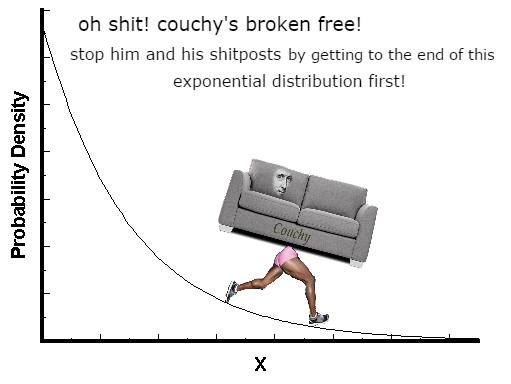
\includegraphics[scale=0.6]{couchy.jpg}

\end{document}